\documentclass[10pt,]{krantz}
\usepackage{lmodern}
\usepackage{amssymb,amsmath}
\usepackage{ifxetex,ifluatex}
\usepackage{fixltx2e} % provides \textsubscript
\ifnum 0\ifxetex 1\fi\ifluatex 1\fi=0 % if pdftex
  \usepackage[T1]{fontenc}
  \usepackage[utf8]{inputenc}
\else % if luatex or xelatex
  \ifxetex
    \usepackage{mathspec}
  \else
    \usepackage{fontspec}
  \fi
  \defaultfontfeatures{Ligatures=TeX,Scale=MatchLowercase}
\fi
% use upquote if available, for straight quotes in verbatim environments
\IfFileExists{upquote.sty}{\usepackage{upquote}}{}
% use microtype if available
\IfFileExists{microtype.sty}{%
\usepackage{microtype}
\UseMicrotypeSet[protrusion]{basicmath} % disable protrusion for tt fonts
}{}
\usepackage[unicode=true]{hyperref}
\PassOptionsToPackage{usenames,dvipsnames}{color} % color is loaded by hyperref
\hypersetup{
            pdftitle={Manual de R},
            colorlinks=true,
            linkcolor=Maroon,
            citecolor=Blue,
            urlcolor=Blue,
            breaklinks=true}
\urlstyle{same}  % don't use monospace font for urls
\usepackage{natbib}
\bibliographystyle{apalike}
\usepackage{color}
\usepackage{fancyvrb}
\newcommand{\VerbBar}{|}
\newcommand{\VERB}{\Verb[commandchars=\\\{\}]}
\DefineVerbatimEnvironment{Highlighting}{Verbatim}{commandchars=\\\{\}}
% Add ',fontsize=\small' for more characters per line
\usepackage{framed}
\definecolor{shadecolor}{RGB}{248,248,248}
\newenvironment{Shaded}{\begin{snugshade}}{\end{snugshade}}
\newcommand{\KeywordTok}[1]{\textcolor[rgb]{0.13,0.29,0.53}{\textbf{{#1}}}}
\newcommand{\DataTypeTok}[1]{\textcolor[rgb]{0.13,0.29,0.53}{{#1}}}
\newcommand{\DecValTok}[1]{\textcolor[rgb]{0.00,0.00,0.81}{{#1}}}
\newcommand{\BaseNTok}[1]{\textcolor[rgb]{0.00,0.00,0.81}{{#1}}}
\newcommand{\FloatTok}[1]{\textcolor[rgb]{0.00,0.00,0.81}{{#1}}}
\newcommand{\ConstantTok}[1]{\textcolor[rgb]{0.00,0.00,0.00}{{#1}}}
\newcommand{\CharTok}[1]{\textcolor[rgb]{0.31,0.60,0.02}{{#1}}}
\newcommand{\SpecialCharTok}[1]{\textcolor[rgb]{0.00,0.00,0.00}{{#1}}}
\newcommand{\StringTok}[1]{\textcolor[rgb]{0.31,0.60,0.02}{{#1}}}
\newcommand{\VerbatimStringTok}[1]{\textcolor[rgb]{0.31,0.60,0.02}{{#1}}}
\newcommand{\SpecialStringTok}[1]{\textcolor[rgb]{0.31,0.60,0.02}{{#1}}}
\newcommand{\ImportTok}[1]{{#1}}
\newcommand{\CommentTok}[1]{\textcolor[rgb]{0.56,0.35,0.01}{\textit{{#1}}}}
\newcommand{\DocumentationTok}[1]{\textcolor[rgb]{0.56,0.35,0.01}{\textbf{\textit{{#1}}}}}
\newcommand{\AnnotationTok}[1]{\textcolor[rgb]{0.56,0.35,0.01}{\textbf{\textit{{#1}}}}}
\newcommand{\CommentVarTok}[1]{\textcolor[rgb]{0.56,0.35,0.01}{\textbf{\textit{{#1}}}}}
\newcommand{\OtherTok}[1]{\textcolor[rgb]{0.56,0.35,0.01}{{#1}}}
\newcommand{\FunctionTok}[1]{\textcolor[rgb]{0.00,0.00,0.00}{{#1}}}
\newcommand{\VariableTok}[1]{\textcolor[rgb]{0.00,0.00,0.00}{{#1}}}
\newcommand{\ControlFlowTok}[1]{\textcolor[rgb]{0.13,0.29,0.53}{\textbf{{#1}}}}
\newcommand{\OperatorTok}[1]{\textcolor[rgb]{0.81,0.36,0.00}{\textbf{{#1}}}}
\newcommand{\BuiltInTok}[1]{{#1}}
\newcommand{\ExtensionTok}[1]{{#1}}
\newcommand{\PreprocessorTok}[1]{\textcolor[rgb]{0.56,0.35,0.01}{\textit{{#1}}}}
\newcommand{\AttributeTok}[1]{\textcolor[rgb]{0.77,0.63,0.00}{{#1}}}
\newcommand{\RegionMarkerTok}[1]{{#1}}
\newcommand{\InformationTok}[1]{\textcolor[rgb]{0.56,0.35,0.01}{\textbf{\textit{{#1}}}}}
\newcommand{\WarningTok}[1]{\textcolor[rgb]{0.56,0.35,0.01}{\textbf{\textit{{#1}}}}}
\newcommand{\AlertTok}[1]{\textcolor[rgb]{0.94,0.16,0.16}{{#1}}}
\newcommand{\ErrorTok}[1]{\textcolor[rgb]{0.64,0.00,0.00}{\textbf{{#1}}}}
\newcommand{\NormalTok}[1]{{#1}}
\usepackage{longtable,booktabs}
\usepackage{graphicx,grffile}
\makeatletter
\def\maxwidth{\ifdim\Gin@nat@width>\linewidth\linewidth\else\Gin@nat@width\fi}
\def\maxheight{\ifdim\Gin@nat@height>\textheight\textheight\else\Gin@nat@height\fi}
\makeatother
% Scale images if necessary, so that they will not overflow the page
% margins by default, and it is still possible to overwrite the defaults
% using explicit options in \includegraphics[width, height, ...]{}
\setkeys{Gin}{width=\maxwidth,height=\maxheight,keepaspectratio}
\IfFileExists{parskip.sty}{%
\usepackage{parskip}
}{% else
\setlength{\parindent}{0pt}
\setlength{\parskip}{6pt plus 2pt minus 1pt}
}
\setlength{\emergencystretch}{3em}  % prevent overfull lines
\providecommand{\tightlist}{%
  \setlength{\itemsep}{0pt}\setlength{\parskip}{0pt}}
\setcounter{secnumdepth}{5}
% Redefines (sub)paragraphs to behave more like sections
\ifx\paragraph\undefined\else
\let\oldparagraph\paragraph
\renewcommand{\paragraph}[1]{\oldparagraph{#1}\mbox{}}
\fi
\ifx\subparagraph\undefined\else
\let\oldsubparagraph\subparagraph
\renewcommand{\subparagraph}[1]{\oldsubparagraph{#1}\mbox{}}
\fi
\usepackage{booktabs}
\usepackage[spanish]{babel}
\decimalpoint
\selectlanguage{spanish}

% Comandos para escribir nombres de paquetes, programas y codigos
\newcommand{\pkg}[1]{{\normalfont\fontseries{b}\selectfont #1}}
\let\proglang=\textsf
\let\code=\texttt


\usepackage{booktabs}
\usepackage{longtable}
\usepackage[bf,singlelinecheck=off]{caption}

\usepackage{framed,color}
\definecolor{shadecolor}{RGB}{248,248,248}

\renewcommand{\textfraction}{0.05}
\renewcommand{\topfraction}{0.8}
\renewcommand{\bottomfraction}{0.8}
\renewcommand{\floatpagefraction}{0.75}

\renewenvironment{quote}{\begin{VF}}{\end{VF}}
\let\oldhref\href
\renewcommand{\href}[2]{#2\footnote{\url{#1}}}

\ifxetex
  \usepackage{letltxmacro}
  \setlength{\XeTeXLinkMargin}{1pt}
  \LetLtxMacro\SavedIncludeGraphics\includegraphics
  \def\includegraphics#1#{% #1 catches optional stuff (star/opt. arg.)
    \IncludeGraphicsAux{#1}%
  }%
  \newcommand*{\IncludeGraphicsAux}[2]{%
    \XeTeXLinkBox{%
      \SavedIncludeGraphics#1{#2}%
    }%
  }%
\fi

\makeatletter
\newenvironment{kframe}{%
\medskip{}
\setlength{\fboxsep}{.8em}
 \def\at@end@of@kframe{}%
 \ifinner\ifhmode%
  \def\at@end@of@kframe{\end{minipage}}%
  \begin{minipage}{\columnwidth}%
 \fi\fi%
 \def\FrameCommand##1{\hskip\@totalleftmargin \hskip-\fboxsep
 \colorbox{shadecolor}{##1}\hskip-\fboxsep
     % There is no \\@totalrightmargin, so:
     \hskip-\linewidth \hskip-\@totalleftmargin \hskip\columnwidth}%
 \MakeFramed {\advance\hsize-\width
   \@totalleftmargin\z@ \linewidth\hsize
   \@setminipage}}%
 {\par\unskip\endMakeFramed%
 \at@end@of@kframe}
\makeatother

\renewenvironment{Shaded}{\begin{kframe}}{\end{kframe}}

\usepackage{makeidx}
\makeindex

\urlstyle{tt}

\usepackage{amsthm}
\makeatletter
\def\thm@space@setup{%
  \thm@preskip=8pt plus 2pt minus 4pt
  \thm@postskip=\thm@preskip
}
\makeatother

\frontmatter

\title{Manual de R}
\author{Freddy Hernández Barajas\\
Olga Cecilia Usuga Manco}
\date{2017-01-23}

\let\BeginKnitrBlock\begin \let\EndKnitrBlock\end
\begin{document}
\maketitle

% you may need to leave a few empty pages before the dedication page

%\cleardoublepage\newpage\thispagestyle{empty}\null
%\cleardoublepage\newpage\thispagestyle{empty}\null
%\cleardoublepage\newpage
\thispagestyle{empty}

\begin{center}

Gracias a Dios por todo lo que me ha dado.

%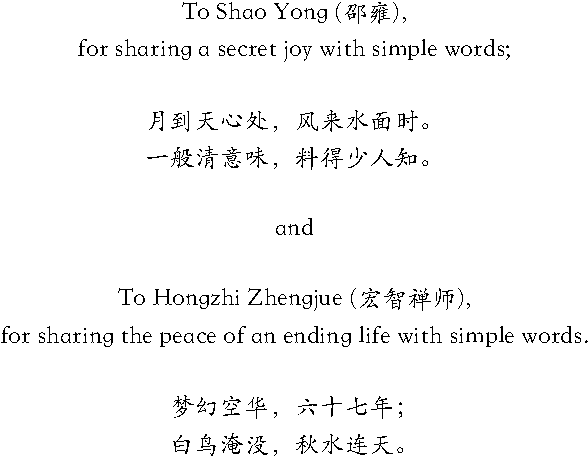
\includegraphics{images/dedication.pdf}
\end{center}

\setlength{\abovedisplayskip}{-5pt}
\setlength{\abovedisplayshortskip}{-5pt}

{
\hypersetup{linkcolor=black}
\setcounter{tocdepth}{2}
\tableofcontents
}
\listoftables
\listoffigures
\chapter*{Prefacio}\label{prefacio}


Este libro fue creado con la intención de apoyar el aprendizaje del
programa \proglang{R} en estudiantes de cualquier pregrado,
especialización, maestría e investigadores que necesiten realizar
análisis estadísticos. El objetivo de este libro es mostrar la forma de
realizar diversos análisis estadísticos, las cuestiones sobre la
creación de gráficos estadísticos no son abordadas en el presente libro,
para consultar sobre gráficos recomendamos consultar
\citet{correa_hernandez}.

\section*{¿Por qué leer este libro?}\label{por-que-leer-este-libro}


Este libro es importante porque \ldots{}

\section*{Estructura del libro}\label{estructura-del-libro}


El libro está estructurado de la siguiente manera.

En el capítulo \ref{central} se muestra como obtener las diversas
medidas de tendencial central para variables cuantitativas, el capítulo
\ref{varia} muestra como calcular las medidas de variabilidad, en el
capítulo \ref{posi} se ilustra cómo usar las funciones para obtener
medidas de posición y en el capítulo \ref{correl} se muestra como
obtener medidas de correlación entre pares de variables.

\section*{Información del software y
convenciones}\label{informacion-del-software-y-convenciones}


Para realizar este libro usamos los paquetes \textbf{knitr}\index{knitr}
\citep{xie2015} y \textbf{bookdown}\index{bookdown} \citep{R-bookdown}.

Package names are in bold text (e.g., \textbf{rmarkdown}), and inline
code and filenames are formatted in a typewriter font (e.g.,
\texttt{knitr::knit(\textquotesingle{}foo.Rmd\textquotesingle{})}).
Function names are followed by parentheses (e.g.,
\texttt{bookdown::render\_book()}).

En todo el libro se presentarán códigos que el lector puede copiar y
pegar en su consola de \proglang{R} para obtener los mismos resultados
aquí presentados. Los códigos se destacan en una caja de color beis (o
beige) similar a la mostrada a continuación.

\begin{Shaded}
\begin{Highlighting}[]
\DecValTok{4} \NormalTok{+}\StringTok{ }\DecValTok{6}
\NormalTok{a <-}\StringTok{ }\KeywordTok{c}\NormalTok{(}\DecValTok{1}\NormalTok{, }\DecValTok{5}\NormalTok{, }\DecValTok{6}\NormalTok{)}
\DecValTok{5} \NormalTok{*}\StringTok{ }\NormalTok{a}
\DecValTok{1}\NormalTok{:}\DecValTok{10}
\end{Highlighting}
\end{Shaded}

Los resultados o salidas obtenidos de cualquier código se destacan con
dos símbolos de númeral (\texttt{\#\#}) al inicio de cada línea o
renglón, esto quiere decir que todo lo que inicie con \texttt{\#\#} son
resultados obtenidos y \textbf{NO} los debe copiar. Abajo se muestran
los resultados obtenidos luego de correr el código anterior.

\begin{verbatim}
## [1] 10
\end{verbatim}

\begin{verbatim}
## [1]  5 25 30
\end{verbatim}

\begin{verbatim}
##  [1]  1  2  3  4  5  6  7  8  9 10
\end{verbatim}

\section*{Agradecimientos}\label{agradecimientos}


Agradecemos enormemente a todos los estudiantes, profesores e
investigadores que han leído este libro y nos han retroalimentado con
comentarios valiosos para mejorar el documento.

\BeginKnitrBlock{flushright}
Freddy Hernández Barajas

Olga Cecilia Usuga Manco
\EndKnitrBlock{flushright}

\chapter*{Sobre los autores}\label{sobre-los-autores}


Freddy Hernández Barajas es profesor asistente de la Universidad
Nacional de Colombia adscrito a la Escuela de Estadística de la Facultad
de Ciencias.

Olga Cecilia Usuga Manco es profesora asociada de la Universidad de
Antioquia adscrita a la Facultad de Ingeniería.

\mainmatter

\chapter{Introducción}\label{introduccion}

\section{Orígenes} \label{sec:origenes}

\proglang{R} es un lenguaje de programación usado para realizar
procedimientos estadísticos y gráficos de alto nivel, este lenguaje fue
creado en 1993 por los profesores e investigadores Robert Gentleman y
Ross Ihaka. Inicialmente el lenguaje se usó para apoyar los cursos que
tenían a su cargo los profesores, pero luego de ver la utilidad de la
herramienta desarrollada, decidieron colocar copias de \proglang{R} en
StatLib. A partir de 1995 el código fuente de \proglang{R} está
disponible bajo licencia GNU GPL para sistemas operativos Windows,
Macintosh y distribuciones Unix/Linux. La comunidad de usuarios de
\proglang{R} en el mundo es muy grande y los usuarios cuentan con
diferentes espacios para interactuar, a continuación una lista no
exhaustiva de los sitios más populares relacionados con \proglang{R}:

\begin{itemize}
\tightlist
\item
  \href{https://www.r-bloggers.com/}{Rbloggers}.
\item
  \href{http://r-es.org/}{Comunidad hispana de \proglang{R}}.
\item
  \href{http://r.789695.n4.nabble.com/}{Nabble}.
\item
  \href{http://r-br.2285057.n4.nabble.com/}{Foro en portugués}.
\item
  \href{http://stackoverflow.com/questions/tagged/r}{Stackoverflow}.
\item
  \href{http://stats.stackexchange.com/questions/tagged/r}{Cross
  Validated}.
\item
  \href{https://stat.ethz.ch/mailman/listinfo/r-help}{\proglang{R}-Help
  Mailing List}.
\item
  \href{http://blog.revolutionanalytics.com/}{Revolutions}.
\item
  \href{https://www.r-statistics.com/}{\proglang{R}-statistics blog}.
\item
  \href{https://rdatamining.wordpress.com/}{RDataMining}.
\end{itemize}

\begin{figure}

{\centering 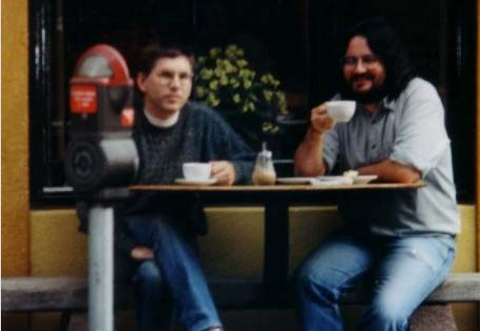
\includegraphics[width=2.4in]{images/Robert_Roos} 

}

\caption{Robert Gentleman (izquierda) y Ross Ihaka (derecha) creadores de R.}\label{fig:unnamed-chunk-4}
\end{figure}

\section{Descarga e instalación} \label{sec:descarga}

Para realizar la instalación de \proglang{R} usted debe visitar la
página del CRAN (\textit{Comprehensive R Archive Network}) disponible en
este \href{https://cran.r-project.org/}{enlace}. Una vez ingrese a la
página encontrará un cuadro similar al mostrado en la Figura
\ref{fig:cran} donde aparecen los enlaces de la instalación para los
sistemas operativos Linux, Mac y Windows.

\begin{figure}

{\centering 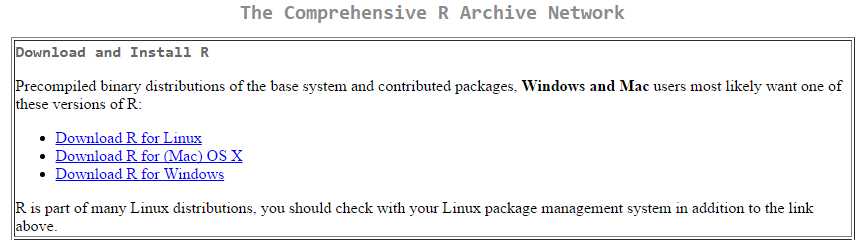
\includegraphics[width=4.54in]{images/cran} 

}

\caption{Página del Cran.}\label{fig:cran}
\end{figure}

Supongamos que se desea instalar \proglang{R} en Windows, para esto se
debe dar clic sobre el hiperenlace
\textcolor{BurntOrange}{Download R for Windows} de la Figura
\ref{fig:cran}. Una vez hecho esto se abrirá una página con el contenido
mostrado en la Figura \ref{fig:inst1}. Una vez ingrese a esa nueva
página usted debe dar clic sobre el hiperenlace
\textcolor{BurntOrange}{install R for the first time} como es señalado
por la flecha roja en la Figura \ref{fig:inst1}.

\begin{figure}

{\centering 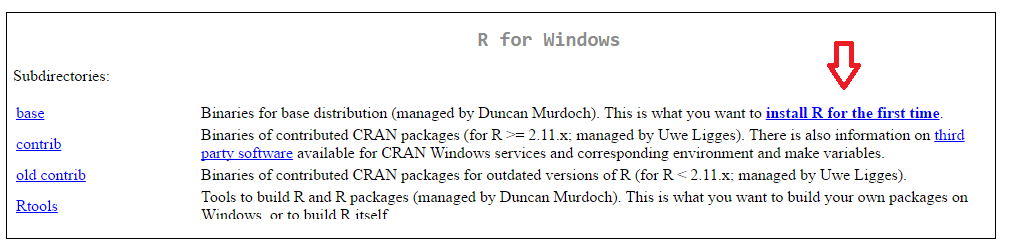
\includegraphics[width=5.31in]{images/instalacion1} 

}

\caption{Página de instalación para la primera ocasión.}\label{fig:inst1}
\end{figure}

Luego de esto se abrirá otra página con un encabezado similar al
mostrado en la Figura \ref{fig:inst2}, al momento de capturar la figura
la versión actual de \proglang{R} era 3.2.5 pero seguramente en este
momento usted tendrá disponible una versión actualizada. Una vez allí
uste debe dar clic sobre
\textcolor{BurntOrange}{Download R 3.2.5 for Windows} como es señalado
por la flecha verde. Luego de esto se descargará el instalador
\proglang{R} en el computador el cual deberá ser instalado con las
opciones que vienen por defecto.

\begin{figure}

{\centering 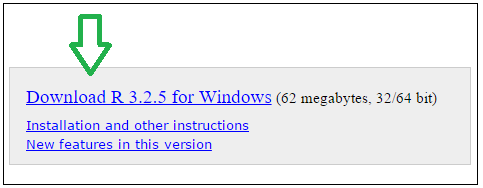
\includegraphics[width=2.54in]{images/instalacion2} 

}

\caption{Página de descarga.}\label{fig:inst2}
\end{figure}

Se recomienda observar el siguiente video didáctico de instalación de
\proglang{R} disponible en este
\href{http://tinyurl.com/jd7b9ks}{enlace} para facilitar la tarea de
instalación.

\section{Apariencia del programa} \label{sec:apariencia}

Una vez que esté instalado \proglang{R} en su computador, usted podrá
acceder a él por la lista de programas o por medio del acceso directo
que quedó en el escritorio, en la Figura \ref{fig:rlogo} se muestra la
apariencia del acceso directo para ingresar a \proglang{R}.

\begin{figure}

{\centering 
\includegraphics[width=1.14in]{images/rlogo} 

}

\caption{Apariencia del acceso directo para ingresar a R.}\label{fig:rlogo}
\end{figure}

Al abrir \proglang{R} aparecerá en la pantalla de su computador algo
similar a lo que está en la Figura \ref{fig:pantalla}. La ventana
izquierda se llama consola y es donde se ingresan las instrucciones, una
vez que se construye un gráfico se activa otra ventana llamada ventana
gráfica. Cualquier usuario puede modificar la posición y tamaños de
estas ventanas, puede cambiar el tipo y tamaño de las letras en la
consola, para hacer esto se deben explorar las opciones de
\textit{editar} en la barra de herramientas.

\begin{figure}

{\centering 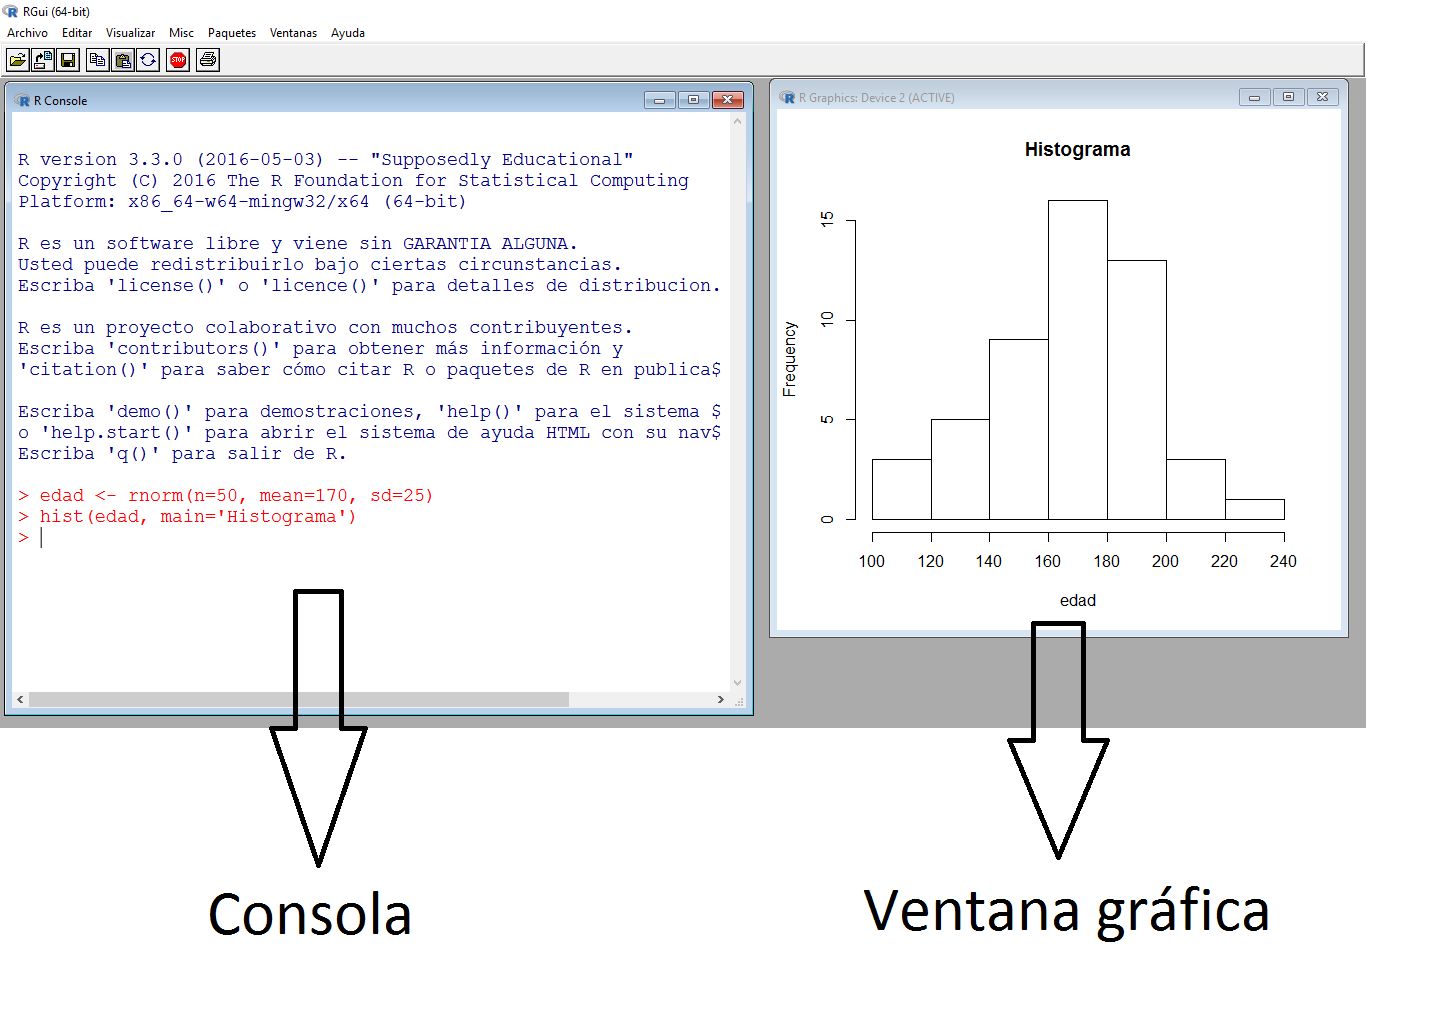
\includegraphics[width=3.6in]{images/Rpantallazo} 

}

\caption{Apariencia de R.}\label{fig:pantalla}
\end{figure}

\section{Tipos de objetos} \label{sec:objetos}

En \proglang{R} existen varios tipos de objectos \index{objetos} que
permiten que el usuario pueda almacenar la información para realizar
procedimientos estadísticos y gráficos. Los principales objetos en
\proglang{R} son vectores, matrices, arreglos, marcos de datos y listas.
A continuación se presentan las características de estos objetos y la
forma para crearlos.

\subsection{Vectores}

Los vectores \index{vectores} son arreglos ordenados en los cuales se
puede almacenar información de tipo numérico (variable cuantitativa),
alfanumérico (variable cualitativa) o lógico (\texttt{TRUE} o
\texttt{FALSE}), pero no mezclas de éstos. La función de \proglang{R}
para crear un vector es \texttt{c()} y que significa concatenar; dentro
de los paréntesis de esta función se ubica la información a almacenar.
Una vez construído el vector se acostumbra a etiquetarlo con un nombre
corto y representativo de la información que almacena, la asignación se
hace por medio del operador \texttt{\textless{}-} entre el nombre y el
vector.

A continuación se presenta un ejemplo de cómo crear tres vectores que
contienen las respuestas de cinco personas a tres preguntas que se les
realizaron.

\begin{Shaded}
\begin{Highlighting}[]
\NormalTok{edad <-}\StringTok{ }\KeywordTok{c}\NormalTok{(}\DecValTok{15}\NormalTok{, }\DecValTok{19}\NormalTok{, }\DecValTok{13}\NormalTok{, }\OtherTok{NA}\NormalTok{, }\DecValTok{20}\NormalTok{)}
\NormalTok{deporte <-}\StringTok{ }\KeywordTok{c}\NormalTok{(}\OtherTok{TRUE}\NormalTok{, }\OtherTok{TRUE}\NormalTok{, }\OtherTok{NA}\NormalTok{, }\OtherTok{FALSE}\NormalTok{, }\OtherTok{TRUE}\NormalTok{)}
\NormalTok{comic.fav <-}\StringTok{ }\KeywordTok{c}\NormalTok{(}\OtherTok{NA}\NormalTok{, }\StringTok{'Superman'}\NormalTok{, }\StringTok{'Batman'}\NormalTok{, }\OtherTok{NA}\NormalTok{, }\StringTok{'Batman'}\NormalTok{)}
\end{Highlighting}
\end{Shaded}

El vector \texttt{edad} es un vector cuantitativo y contiene las edades
de las 5 personas. En la cuarta posición del vector se colocó el símbolo
\texttt{NA} que significa \textit{Not Available} debido a que no se
registró la edad para esa persona. Al hacer una asignación se acostumbra
a dejar un espacio antes y después del operador \texttt{\textless{}-} de
asignación. El segundo vector es llamado \texttt{deporte} y es un vector
lógico que almacena las respuestas a la pregunta de si la persona
practica deporte, nuevamente aquí hay un \texttt{NA} para la tercera
persona. El último vector \texttt{comic.fav} contiene la información del
cómic favorito de cada persona, como esta variable es cualitativa es
necesario usar las comillas
\texttt{\textquotesingle{}\ \textquotesingle{}} para encerrar las
respuestas. Cuando se usa \texttt{NA} para representar una información
\textit{Not Available} NO SE DEBEN usar las comillas
\texttt{\textquotesingle{}\ \textquotesingle{}}.

Nota: es posible usar comillas sencillas
\texttt{\textquotesingle{}foo\textquotesingle{}} o comillas dobles
\texttt{"foo"} para ingresar valores de una variable cualitativa.

Si se desea ver lo que está almacenado en cada uno de estos vectores, se
debe escribir en la consola de \proglang{R} el nombre de uno de los
objetos y luego se presiona la tecla \textit{enter} o \textit{intro}, al
realizar esto lo que se obtiene se muestra a continuación.

\begin{Shaded}
\begin{Highlighting}[]
\NormalTok{edad}
\end{Highlighting}
\end{Shaded}

\begin{verbatim}
## [1] 15 19 13 NA 20
\end{verbatim}

\begin{Shaded}
\begin{Highlighting}[]
\NormalTok{deporte}
\end{Highlighting}
\end{Shaded}

\begin{verbatim}
## [1]  TRUE  TRUE    NA FALSE  TRUE
\end{verbatim}

\begin{Shaded}
\begin{Highlighting}[]
\NormalTok{comic.fav}
\end{Highlighting}
\end{Shaded}

\begin{verbatim}
## [1] NA         "Superman" "Batman"   NA        
## [5] "Batman"
\end{verbatim}

\subsection{Matrices}

Las matrices \index{matrices} son arreglos rectangulares de filas y
columnas con información numérica, alfanumérica o lógica. Para construir
una matriz se usa la función \texttt{matrix(\ )}. Por ejemplo, para
crear una matriz de 4 filas y 5 columnas (de dimensión \(4 \times 5\))
con los primeros 20 números positivos se escribe el código siguiente en
la consola.

\begin{Shaded}
\begin{Highlighting}[]
\NormalTok{mimatriz <-}\StringTok{ }\KeywordTok{matrix}\NormalTok{(}\DataTypeTok{data=}\DecValTok{1}\NormalTok{:}\DecValTok{20}\NormalTok{, }\DataTypeTok{nrow=}\DecValTok{4}\NormalTok{, }\DataTypeTok{ncol=}\DecValTok{5}\NormalTok{, }\DataTypeTok{byrow=}\OtherTok{FALSE}\NormalTok{)}
\end{Highlighting}
\end{Shaded}

El argumento \texttt{data} de la función sirve para indicar los datos
que se van a almacenar en la matriz, los argumentos \texttt{nrow} y
\texttt{ncol} sirven para definir la dimensión de la matriz y por último
el argumento \texttt{byrow} sirve para indicar si la información
contenida en \texttt{data} se debe ingresar por filas o no. Para
observar lo que quedó almacenado en el objeto \texttt{mimatriz} se
escribe en la consola el nombre del objeto seguido de la tecla
\textit{enter} o \textit{intro}.

\begin{Shaded}
\begin{Highlighting}[]
\NormalTok{mimatriz}
\end{Highlighting}
\end{Shaded}

\begin{verbatim}
##      [,1] [,2] [,3] [,4] [,5]
## [1,]    1    5    9   13   17
## [2,]    2    6   10   14   18
## [3,]    3    7   11   15   19
## [4,]    4    8   12   16   20
\end{verbatim}

\subsection{Arreglos}

Un arreglo \index{arreglo} es una matriz de varias dimensiones con
información numérica, alfanumérica o lógica. Para construir una arreglo
se usa la función \texttt{array(\ )}. Por ejemplo, para crear un arreglo
de \(3 \times 4 \times 2\) con las primeras 24 letras minúsculas del
alfabeto se escribe el siguiente código.

\begin{Shaded}
\begin{Highlighting}[]
\NormalTok{miarray <-}\StringTok{ }\KeywordTok{array}\NormalTok{(}\DataTypeTok{data=}\NormalTok{letters[}\DecValTok{1}\NormalTok{:}\DecValTok{24}\NormalTok{], }\DataTypeTok{dim=}\KeywordTok{c}\NormalTok{(}\DecValTok{3}\NormalTok{, }\DecValTok{4}\NormalTok{, }\DecValTok{2}\NormalTok{))}
\end{Highlighting}
\end{Shaded}

El argumento \texttt{data} de la función sirve para indicar los datos
que se van a almacenar en el arreglo y el argumento \texttt{dim} sirve
para indicar las dimensiones del arreglo. Para observar lo que quedó
almacenado en el objeto \texttt{miarray} se escribe en la consola lo
siguiente.

\begin{Shaded}
\begin{Highlighting}[]
\NormalTok{miarray}
\end{Highlighting}
\end{Shaded}

\begin{verbatim}
## , , 1
## 
##      [,1] [,2] [,3] [,4]
## [1,] "a"  "d"  "g"  "j" 
## [2,] "b"  "e"  "h"  "k" 
## [3,] "c"  "f"  "i"  "l" 
## 
## , , 2
## 
##      [,1] [,2] [,3] [,4]
## [1,] "m"  "p"  "s"  "v" 
## [2,] "n"  "q"  "t"  "w" 
## [3,] "o"  "r"  "u"  "x"
\end{verbatim}

\subsection{Marco de datos}

El marco de datos \index{marco de datos} o \textit{data frame} es uno de
los objetos más utilizados porque permite agrupar vectores con
información de diferente tipo (numérica, alfanumérica o lógica) en un
mismo objeto, la única restricción es que los vectores deben tener la
misma longitud. Para crear un marco de datos se usa la función
\texttt{data.frame(\ )}, como ejemplo vamos a crear un marco de datos
con los vectores \texttt{edad}, \texttt{deporte} y \texttt{comic.fav}
definidos anteriormente.

\begin{Shaded}
\begin{Highlighting}[]
\NormalTok{mimarco <-}\StringTok{ }\KeywordTok{data.frame}\NormalTok{(edad, deporte, comic.fav)}
\end{Highlighting}
\end{Shaded}

Una vez creado el objeto \texttt{mimarco} podemos ver el objeto
escribiendo su nombre en la consola, a continuación se muestra lo que se
obtiene.

\begin{Shaded}
\begin{Highlighting}[]
\NormalTok{mimarco}
\end{Highlighting}
\end{Shaded}

\begin{verbatim}
##   edad deporte comic.fav
## 1   15    TRUE      <NA>
## 2   19    TRUE  Superman
## 3   13      NA    Batman
## 4   NA   FALSE      <NA>
## 5   20    TRUE    Batman
\end{verbatim}

De la salida anterior vemos que el marco de datos tiene 3 variables
(columnas) cuyos nombres coinciden con los nombres de los vectores
creados anteriormente, los números consecutivos al lado izquierdo son
sólo de referencia y permiten identificar la información para cada
persona en la base de datos.

\subsection{Listas}

Las listas \index{lista} son otro tipo de objeto muy usado para
almacenar objetos de diferente tipo. La instrucción para crear una lista
es \texttt{list(\ )}. A continuación vamos a crear una lista que
contiene tres objetos: un vector con 5 números aleatorios llamado
\texttt{mivector}, una matriz de dimensión \(6 \times 2\) con los
primeros doce números enteros positivos llamada \texttt{matriz2} y el
tercer objeto será el marco de datos \texttt{mimarco} creado en el
apartado anterior. Las instrucciones para crear la lista requerida se
muestran a continuación.

\begin{Shaded}
\begin{Highlighting}[]
\KeywordTok{set.seed}\NormalTok{(}\DecValTok{12345}\NormalTok{)}
\NormalTok{mivector <-}\StringTok{ }\KeywordTok{runif}\NormalTok{(}\DataTypeTok{n=}\DecValTok{5}\NormalTok{)}
\NormalTok{matriz2 <-}\StringTok{ }\KeywordTok{matrix}\NormalTok{(}\DataTypeTok{data=}\DecValTok{1}\NormalTok{:}\DecValTok{12}\NormalTok{, }\DataTypeTok{ncol=}\DecValTok{6}\NormalTok{)}
\NormalTok{milista <-}\StringTok{ }\KeywordTok{list}\NormalTok{(}\DataTypeTok{E1=}\NormalTok{mivector, }\DataTypeTok{E2=}\NormalTok{matriz2, }\DataTypeTok{E3=}\NormalTok{mimarco)}
\end{Highlighting}
\end{Shaded}

La función \texttt{set.seed} de la línea número 1 sirve para fijar la
semilla de tal manera que los números aleatorios generados en la segunda
línea con la función \texttt{runif} sean siempre los mismos. En la
última línea del código anterior se construye la lista, dentro de la
función \texttt{list} se colocan los tres objetos \texttt{mivector},
\texttt{matriz2} y \texttt{mimarco}. Es posible colocarle un nombre
especial a cada uno de los elementos de la lista, en este ejemplo se
colocaron los nombres \texttt{E1}, \texttt{E2} y \texttt{E3} para cada
uno de los tres elementos. Para observar lo que quedó almacenado en la
lista se escribe \texttt{milista} en la consola y el resultado se
muestra a continuación.

\begin{Shaded}
\begin{Highlighting}[]
\NormalTok{milista}
\end{Highlighting}
\end{Shaded}

\begin{verbatim}
## $E1
## [1] 0.7209 0.8758 0.7610 0.8861 0.4565
## 
## $E2
##      [,1] [,2] [,3] [,4] [,5] [,6]
## [1,]    1    3    5    7    9   11
## [2,]    2    4    6    8   10   12
## 
## $E3
##   edad deporte comic.fav
## 1   15    TRUE      <NA>
## 2   19    TRUE  Superman
## 3   13      NA    Batman
## 4   NA   FALSE      <NA>
## 5   20    TRUE    Batman
\end{verbatim}

\section{Guía de estilo para la escritura en R} \label{sec:estilo}

Así como en el español existen reglas ortográficas, la escritura de
códigos en \proglang{R} también tiene unas reglas que se recomienda
seguir para evitar confusiones. Tener una buena guía de estilo
\index{guía de estilo} es importante para que el código creado por usted
sea fácilmente entendido por sus lectores \citet{rpackages}. No existe
una única y mejor guía de estilo para escritura en \proglang{R}, sin
embargo aquí vamos a mostrar unas sugerencias basadas en la guía llamada
\href{https://google.github.io/styleguide/Rguide.xml}{\textit{Google's R style guide}}.

\subsection{Nombres de los archivos}

Se sugiere que el nombre usado para nombrar un archivo tenga sentido y
que termine con extensión .R. A continuación dos ejemplos de como
nombrar mal y bien un archivo.

\begin{itemize}
    \item Mal: \verb|hola.R|
    \item Bien: \verb|analisis_icfes.R|
\end{itemize}

\subsection{Nombres de los objetos}

Se recomienda no usar los símbolos \texttt{\_} y \texttt{-} dentro de
los nombres de objetos. Para las variables es preferible usar letras
minúsculas y separar las palabras con puntos (\texttt{peso.maiz}) o
utilizar la notación camello iniciando en minúscula (\texttt{pesoMaiz}).
Para las funciones se recomienda usar la notación camello iniciando
todas la palabras en mayúscula (\texttt{PlotRes}). Para los nombres de
las constantes se recomienda que inicien con la letra k
(\texttt{kPrecioBus}). A continuación ejemplos de buenas y malas
prácticas.

Para variables:

\begin{itemize}
    \item Bien: \verb|avg.clicks|
    \item Aceptable: \verb|avgClicks|
    \item Mal: \verb|avg_Clicks|
\end{itemize}

Para funciones:

\begin{itemize}
    \item Bien: \verb|CalculateAvgClicks| 
    \item Mal: \verb|calculate_avg_clicks| , \verb|calculateAvgClicks|
\end{itemize}

\subsection{Longitud de una línea de código}

Se recomienda que cada línea tenga como máximo 80 caracteres. Si una
línea es muy larga se debe cortar siempre por una coma.

\subsection{Espacios}

Use espacios alrededor de todos los operadores binarios (=, +, -,
\textless{}-, etc.). Los espacios alrededor del símbolo ``='' son
opcionales cuando se usan para ingresar valores dentro de una función.
Así como en español, nunca coloque espacio antes de una coma, pero
siempre use espacio luego de una coma. A continuación ejemplos de buenas
y malas prácticas.

\begin{Shaded}
\begin{Highlighting}[]
\NormalTok{tab <-}\StringTok{ }\KeywordTok{table}\NormalTok{(df[df$days <}\StringTok{ }\DecValTok{0}\NormalTok{, }\DecValTok{2}\NormalTok{])  }\CommentTok{# Bien}
\NormalTok{tot <-}\StringTok{ }\KeywordTok{sum}\NormalTok{(x[, }\DecValTok{1}\NormalTok{])                }\CommentTok{# Bien}
\NormalTok{tot <-}\StringTok{ }\KeywordTok{sum}\NormalTok{(x[}\DecValTok{1}\NormalTok{, ])                }\CommentTok{# Bien}
\NormalTok{tab <-}\StringTok{ }\KeywordTok{table}\NormalTok{(df[df$days<}\DecValTok{0}\NormalTok{, }\DecValTok{2}\NormalTok{])    }\CommentTok{# Faltan espacios alrededor '<' }
\NormalTok{tab <-}\StringTok{ }\KeywordTok{table}\NormalTok{(df[df$days <}\StringTok{ }\DecValTok{0}\NormalTok{,}\DecValTok{2}\NormalTok{])   }\CommentTok{# Falta espacio luego de coma}
\NormalTok{tab <-}\StringTok{ }\KeywordTok{table}\NormalTok{(df[df$days <}\StringTok{ }\DecValTok{0} \NormalTok{, }\DecValTok{2}\NormalTok{]) }\CommentTok{# Sobra espacio antes de coma}
\NormalTok{tab<-}\StringTok{ }\KeywordTok{table}\NormalTok{(df[df$days <}\StringTok{ }\DecValTok{0}\NormalTok{, }\DecValTok{2}\NormalTok{])   }\CommentTok{# Falta espacio antes de '<-'}
\NormalTok{tab<-}\KeywordTok{table}\NormalTok{(df[df$days <}\StringTok{ }\DecValTok{0}\NormalTok{, }\DecValTok{2}\NormalTok{])    }\CommentTok{# Falta espacio alrededor de '<-'}
\NormalTok{tot <-}\StringTok{ }\KeywordTok{sum}\NormalTok{(x[,}\DecValTok{1}\NormalTok{])                 }\CommentTok{# Falta espacio luego de coma}
\NormalTok{tot <-}\StringTok{ }\KeywordTok{sum}\NormalTok{(x[}\DecValTok{1}\NormalTok{,])                 }\CommentTok{# Falta espacio luego de coma}
\end{Highlighting}
\end{Shaded}

Otra buena práctica es colocar espacio antes de un paréntesis excepto
cuando se llama una función.

\begin{Shaded}
\begin{Highlighting}[]
\NormalTok{if (debug)    }\CommentTok{# Correcto}
\NormalTok{if(debug)     }\CommentTok{# Funciona pero no se recomienda}
\KeywordTok{colMeans} \NormalTok{(x)  }\CommentTok{# Funciona pero no se recomienda}
\end{Highlighting}
\end{Shaded}

Espacios extras pueden ser usados si con esto se mejora la apariencia
del código, ver el ejemplo siguiente.

\begin{Shaded}
\begin{Highlighting}[]
\KeywordTok{plot}\NormalTok{(}\DataTypeTok{x    =} \NormalTok{x.coord,}
     \DataTypeTok{y    =} \NormalTok{data.mat[, }\KeywordTok{MakeColName}\NormalTok{(metric, ptiles[}\DecValTok{1}\NormalTok{], }\StringTok{"roiOpt"}\NormalTok{)],}
     \DataTypeTok{ylim =} \NormalTok{ylim,}
     \DataTypeTok{xlab =} \StringTok{"dates"}\NormalTok{,}
     \DataTypeTok{ylab =} \NormalTok{metric,}
     \DataTypeTok{main =} \NormalTok{(}\KeywordTok{paste}\NormalTok{(metric, }\StringTok{" for 3 samples "}\NormalTok{, }\DataTypeTok{sep =} \StringTok{""}\NormalTok{)))}
\end{Highlighting}
\end{Shaded}

No coloque espacios alrededor del código que esté dentro de paréntesis
\texttt{(\ )} o corchetes \texttt{{[}\ {]}}, la única excepción es luego
de una coma, ver el ejemplo siguiente.

\begin{Shaded}
\begin{Highlighting}[]
\NormalTok{if (condicion)    }\CommentTok{# Correcto }
\NormalTok{x[}\DecValTok{1}\NormalTok{, ]            }\CommentTok{# Correcto}
\NormalTok{if ( condicion )  }\CommentTok{# Sobran espacios alrededor de condicion}
\NormalTok{x[}\DecValTok{1}\NormalTok{,]             }\CommentTok{# Se necesita espacio luego de coma}
\end{Highlighting}
\end{Shaded}

Los signos de agrupación llaves \texttt{\{\ \}} se utilizan para agrupar
bloques de código y se recomienda que nunca una llave abierta
\texttt{\{} esté sola en una línea; una llave cerrada \texttt{\}} si
debe ir sola en su propia línea. Se pueden omitir las llaves cuando el
bloque de instrucciones esté formado por una sola línea pero esa línea
de código NO debe ir en la misma línea de la condición. A continuación
dos ejemplos de lo que se recomienda.

\begin{Shaded}
\begin{Highlighting}[]
\NormalTok{if (}\KeywordTok{is.null}\NormalTok{(ylim)) \{                     }\CommentTok{# Correcto}
  \NormalTok{ylim <-}\StringTok{ }\KeywordTok{c}\NormalTok{(}\DecValTok{0}\NormalTok{, }\FloatTok{0.06}\NormalTok{)}
\NormalTok{\}}

\NormalTok{if (}\KeywordTok{is.null}\NormalTok{(ylim))                       }\CommentTok{# Correcto}
  \NormalTok{ylim <-}\StringTok{ }\KeywordTok{c}\NormalTok{(}\DecValTok{0}\NormalTok{, }\FloatTok{0.06}\NormalTok{)}

\NormalTok{if (}\KeywordTok{is.null}\NormalTok{(ylim)) ylim <-}\StringTok{ }\KeywordTok{c}\NormalTok{(}\DecValTok{0}\NormalTok{, }\FloatTok{0.06}\NormalTok{)    }\CommentTok{# Aceptable}

\NormalTok{if (}\KeywordTok{is.null}\NormalTok{(ylim))                       }\CommentTok{# No se recomienda}
\NormalTok{\{        }
  \NormalTok{ylim <-}\StringTok{ }\KeywordTok{c}\NormalTok{(}\DecValTok{0}\NormalTok{, }\FloatTok{0.06}\NormalTok{)}
\NormalTok{\}}
    
\NormalTok{if (}\KeywordTok{is.null}\NormalTok{(ylim)) \{ylim <-}\StringTok{ }\KeywordTok{c}\NormalTok{(}\DecValTok{0}\NormalTok{, }\FloatTok{0.06}\NormalTok{)\}}
\CommentTok{# Frente a la llave \{ no debe ir nada}
\CommentTok{# la llave de cierre \} debe ir sola}
\end{Highlighting}
\end{Shaded}

La sentencia else debe ir siempre entre llaves \texttt{\}\ \{}, ver el
siguiente ejemplo.

\begin{Shaded}
\begin{Highlighting}[]
\NormalTok{if (condition) \{         }
  \NormalTok{one or more lines}
\NormalTok{\} else \{                 }\CommentTok{# Correcto}
  \NormalTok{one or more lines}
\NormalTok{\}}


\NormalTok{if (condition) \{         }
  \NormalTok{one or more lines}
\NormalTok{\}}
\NormalTok{else \{                   }\CommentTok{# Incorrecto}
  \NormalTok{one or more lines}
\NormalTok{\}}


\NormalTok{if (condition)           }
  \NormalTok{one line}
\NormalTok{else                     }\CommentTok{# Incorrecto}
  \NormalTok{one line}
\end{Highlighting}
\end{Shaded}

\subsection{Asignación}

Para realizar asignaciones se recomienda usar el símbolo
\texttt{\textless{}-}, el símbolo de igualdad \texttt{=} no se
recomienda usarlo para asignaciones.

\begin{Shaded}
\begin{Highlighting}[]
\NormalTok{x <-}\StringTok{ }\DecValTok{5}  \CommentTok{# Correcto}
\NormalTok{x =}\StringTok{ }\DecValTok{5}   \CommentTok{# No recomendado}
\end{Highlighting}
\end{Shaded}

Para una explicación más detallada sobre el símbolo de asignación se
recomienda visitar este
\href{http://www.win-vector.com/blog/2016/12/the-case-for-using-in-r/}{enlace}.

\subsection{Punto y coma}

No se recomienda colocar varias instrucciones separadas por \texttt{;}
en la misma línea, aunque funciona dificulta la revisión del código.

\begin{Shaded}
\begin{Highlighting}[]
\NormalTok{n <-}\StringTok{ }\DecValTok{100}\NormalTok{; y <-}\StringTok{ }\KeywordTok{rnorm}\NormalTok{(n, }\DataTypeTok{mean=}\DecValTok{5}\NormalTok{); }\KeywordTok{hist}\NormalTok{(y)  }\CommentTok{# No se recomienda}

\NormalTok{n <-}\StringTok{ }\DecValTok{100}                                  \CommentTok{# Correcto}
\NormalTok{y <-}\StringTok{ }\KeywordTok{rnorm}\NormalTok{(n, }\DataTypeTok{mean=}\DecValTok{5}\NormalTok{)}
\KeywordTok{hist}\NormalTok{(y)}
\end{Highlighting}
\end{Shaded}

A pesar de la anterior advertencia es posible que en este libro usemos
el \texttt{;} en algunas ocasiones, si lo hacemos es para ahorrar
espacio en la presentación del código.

\chapter{\texorpdfstring{Medidas de tendencia central
\label{central}}{Medidas de tendencia central }}\label{medidas-de-tendencia-central}

En este capítulo se mostrará cómo obtener las diferentes medidas de
tendencia central con \proglang{R}.

Para ilustrar el uso de las funciones se utilizará una base de datos
llamada \textbf{medidas del cuerpo}, esta base de datos cuenta con 6
variables registradas a un grupo de 36 estudiantes de la universidad.
Las variables son:

\begin{enumerate}
\def\labelenumi{\arabic{enumi}.}
\tightlist
\item
  \texttt{edad} del estudiante (años),
\item
  \texttt{peso} del estudiante (kilogramos),
\item
  \texttt{altura} del estudiante (centímetros),
\item
  \texttt{sexo} del estudiante (Hombre, Mujer),
\item
  \texttt{muneca}: perímetro de la muñeca derecha (centímetros),
\item
  \texttt{biceps}: perímetro del biceps derecho (centímetros).
\end{enumerate}

A continuación se presenta el código para definir la url donde están los
datos, para cargar la base de datos en R y para mostrar por pantalla un
encabezado (usando \texttt{head}) de la base de datos.

\begin{Shaded}
\begin{Highlighting}[]
\NormalTok{url <-}\StringTok{ 'https://raw.githubusercontent.com/fhernanb/datos/master/medidas_cuerpo'}
\NormalTok{datos <-}\StringTok{ }\KeywordTok{read.table}\NormalTok{(}\DataTypeTok{file=}\NormalTok{url, }\DataTypeTok{header=}\NormalTok{T)}
\KeywordTok{head}\NormalTok{(datos)  }\CommentTok{# Para ver el encabezado de la base de datos}
\end{Highlighting}
\end{Shaded}

\begin{verbatim}
##   edad peso altura   sexo muneca biceps
## 1   43 87.3  188.0 Hombre   12.2   35.8
## 2   65 80.0  174.0 Hombre   12.0   35.0
## 3   45 82.3  176.5 Hombre   11.2   38.5
## 4   37 73.6  180.3 Hombre   11.2   32.2
## 5   55 74.1  167.6 Hombre   11.8   32.9
## 6   33 85.9  188.0 Hombre   12.4   38.5
\end{verbatim}

\section{\texorpdfstring{Media \index{media}
\index{mean}}{Media  }}\label{media}

Para calcular la media de una variable cuantitativa se usa la función
\texttt{mean}. Los argumentos básicos de la función \texttt{mean} son
dos y se muestran a continuación.

\begin{Shaded}
\begin{Highlighting}[]
\KeywordTok{mean}\NormalTok{(x, }\DataTypeTok{na.rm =} \OtherTok{FALSE}\NormalTok{)}
\end{Highlighting}
\end{Shaded}

En el parámetro \texttt{x} se indica la variable de interés para la cual
se quiere calcular la media, el parámetro \texttt{na.rm} es un valor
lógico que en caso de ser \texttt{TRUE}, significa que se deben remover
las observaciones con \texttt{NA}, el valor por defecto para este
parámetro es \texttt{FALSE}.

\subsection*{Ejemplo}\label{ejemplo}


Suponga que queremos obtener la altura media del grupo de estudiantes.

Para encontrar la media general se usa la función \texttt{mean} sobre el
vector númerico \texttt{datos\$altura}.

\begin{Shaded}
\begin{Highlighting}[]
\KeywordTok{mean}\NormalTok{(}\DataTypeTok{x=}\NormalTok{datos$altura)}
\end{Highlighting}
\end{Shaded}

\begin{verbatim}
## [1] 171.6
\end{verbatim}

Del anterior resultado podemos decir que la estatura media o promedio de
los estudiantes es 171.5556 centímetros.

\subsection*{Ejemplo}\label{ejemplo-1}


Suponga que ahora queremos la altura media pero diferenciando por sexo.

Para hacer esto se debe primero dividir o partir el vector de altura
según los niveles de la variable sexo, esto se consigue por medio de la
función \texttt{split} y el resultado será una lista con tantos
elementos como niveles tenga la variable sexo. Luego a cada uno de los
elementos de la lista se le aplica la función \texttt{mean} con la ayuda
de \texttt{sapply} o \texttt{tapply}. A continuación el código completo
para obtener las alturas medias para hombres y mujeres.

\begin{Shaded}
\begin{Highlighting}[]
\KeywordTok{sapply}\NormalTok{(}\KeywordTok{split}\NormalTok{(}\DataTypeTok{x=}\NormalTok{datos$altura, }\DataTypeTok{f=}\NormalTok{datos$sexo), mean)}
\end{Highlighting}
\end{Shaded}

\begin{verbatim}
## Hombre  Mujer 
##  179.1  164.0
\end{verbatim}

El resultado es un vector con dos elementos, vemos que la altura media
para hombres es 179.0778 centímetros y que para las mujeres es de
164.0333 centímetros.

¿Qué sucede si se usa \texttt{tapply} en lugar de \texttt{sapply}?
Substituya en el código anterior la función \texttt{sapply} por
\texttt{tapply} y observe la diferencia entre los resultados.

\subsection*{Ejemplo}\label{ejemplo-2}


Suponga que se tiene el vector \texttt{edad} con las edades de siete
personas y supóngase que para el individuo cinco no se tiene información
de su edad, eso significa que el vector tendrá un \texttt{NA} en la
quinta posición.

¿Cuál será la edad promedio del grupo de personas?

\begin{Shaded}
\begin{Highlighting}[]
\NormalTok{edad <-}\StringTok{ }\KeywordTok{c}\NormalTok{(}\DecValTok{18}\NormalTok{, }\DecValTok{23}\NormalTok{, }\DecValTok{26}\NormalTok{, }\DecValTok{32}\NormalTok{, }\OtherTok{NA}\NormalTok{, }\DecValTok{32}\NormalTok{, }\DecValTok{29}\NormalTok{)}
\KeywordTok{mean}\NormalTok{(}\DataTypeTok{x=}\NormalTok{edad)}
\end{Highlighting}
\end{Shaded}

\begin{verbatim}
## [1] NA
\end{verbatim}

Al correr el código anterior se obtiene un error y es debido al símbolo
\texttt{NA} en la quinta posición. Para calcular la media sólo con los
datos de los cuales se tiene información, se incluye el argumento
\texttt{na.rm\ =\ TRUE} para que R remueva los \texttt{NA}. El código
correcto a usar en este caso es:

\begin{Shaded}
\begin{Highlighting}[]
\KeywordTok{mean}\NormalTok{(}\DataTypeTok{x=}\NormalTok{edad, }\DataTypeTok{na.rm=}\OtherTok{TRUE}\NormalTok{)}
\end{Highlighting}
\end{Shaded}

\begin{verbatim}
## [1] 26.67
\end{verbatim}

De este último resultado se obtiene que la edad promedio de los
individuos es 26.67 años.

\section{\texorpdfstring{Mediana \index{mediana}
\index{median}}{Mediana  }}\label{mediana}

Para calcular la mediana de una variable cantitativa se usa la función
\texttt{median}. Los argumentos básicos de la función \texttt{median}
son dos y se muestran a continuación.

\begin{Shaded}
\begin{Highlighting}[]
\KeywordTok{median}\NormalTok{(x, }\DataTypeTok{na.rm =} \OtherTok{FALSE}\NormalTok{)}
\end{Highlighting}
\end{Shaded}

En el parámetro \texttt{x} se indica la variable de interés para la cual
se quiere calcular la mediana, el parámetro \texttt{na.rm} es un valor
lógico que en caso de ser \texttt{TRUE}, significa que se deben remover
las observaciones con \texttt{NA}, el valor por defecto para este
parámetro es \texttt{FALSE}.

\subsection*{Ejemplo}\label{ejemplo-3}


Calcular la edad mediana para los estudiantes de la base de datos.

Para obtener la mediana usamos el siguiente código:

\begin{Shaded}
\begin{Highlighting}[]
\KeywordTok{median}\NormalTok{(}\DataTypeTok{x=}\NormalTok{datos$edad)}
\end{Highlighting}
\end{Shaded}

\begin{verbatim}
## [1] 28
\end{verbatim}

y obtenemos que la mitad de los estudiantes tienen edades mayores o
iguales a 28 años.

El resultado anterior se pudo haber obtenido con la función
\texttt{quantile} e indicando que se desea el cuantil 50 así:

\begin{Shaded}
\begin{Highlighting}[]
\KeywordTok{quantile}\NormalTok{(}\DataTypeTok{x=}\NormalTok{datos$edad, }\DataTypeTok{probs=}\FloatTok{0.5}\NormalTok{)}
\end{Highlighting}
\end{Shaded}

\begin{verbatim}
## 50% 
##  28
\end{verbatim}

\section{\texorpdfstring{Moda \index{moda}}{Moda }}\label{moda}

La moda de una variable cuantitativa corresponde a valor o valores que
más se repiten, una forma sencilla de encontrar la moda es construir una
tabla de frecuencias y observar los valores con mayor frecuencia.

\subsection*{Ejemplo}\label{ejemplo-4}


Calcular la moda para la variable edad de la base de datos de
estudiantes.

Se construye la tabla con la función \texttt{table} y se crea el objeto
\texttt{tabla} para almacenarla.

\begin{Shaded}
\begin{Highlighting}[]
\NormalTok{tabla <-}\StringTok{ }\KeywordTok{table}\NormalTok{(datos$edad)}
\NormalTok{tabla}
\end{Highlighting}
\end{Shaded}

\begin{verbatim}
## 
## 19 20 21 22 23 24 25 26 28 29 30 32 33 35 37 40 43 45 
##  1  1  1  3  2  1  5  3  2  1  2  1  1  2  3  1  2  1 
## 51 55 65 
##  1  1  1
\end{verbatim}

Al mirar con detalle la tabla anterior se observa que el valor que más
se repite es la edad de 25 años en 5 ocasiones. Si la tabla hubiese sido
mayor, la inspección visual nos podría tomar unos segundos o hasta
minutos y podríamos equivocarnos, por esa razón es mejor ordenar los
resultados de la tabla.

Para observar los valores con mayor frecuencia de la tabla se puede
ordenar la tabla usando la función \texttt{sort} de la siguiente manera:

\begin{Shaded}
\begin{Highlighting}[]
\KeywordTok{sort}\NormalTok{(tabla, }\DataTypeTok{decreasing=}\OtherTok{TRUE}\NormalTok{)}
\end{Highlighting}
\end{Shaded}

\begin{verbatim}
## 
## 25 22 26 37 23 28 30 35 43 19 20 21 24 29 32 33 40 45 
##  5  3  3  3  2  2  2  2  2  1  1  1  1  1  1  1  1  1 
## 51 55 65 
##  1  1  1
\end{verbatim}

De esta manera se ve fácilmente que la variable edad es unimodal con
valor de 25 años.

\chapter{\texorpdfstring{Medidas de variabilidad
\label{varia}}{Medidas de variabilidad }}\label{medidas-de-variabilidad}

En este capítulo se mostrará cómo obtener las diferentes medidas de
variabilidad con \proglang{R}.

Para ilustrar el uso de las funciones se utilizará la base de datos
llamada \textbf{aptos2015}, esta base de datos cuenta con 11 variables
registradas a apartamentos usados en la ciudad de Medellín. Las
variables de la base de datos son:

\begin{enumerate}
\def\labelenumi{\arabic{enumi}.}
\tightlist
\item
  \texttt{precio}: precio de venta del apartamento (millones de pesos),
\item
  \texttt{mt2}: área del apartamento (\(m^2\)),
\item
  \texttt{ubicacion}: lugar de ubicación del aparamentos en la ciudad
  (cualitativa),
\item
  \texttt{estrato}: nivel socioeconómico donde está el apartamento (2 a
  6),
\item
  \texttt{alcobas}: número de alcobas del apartamento,
\item
  \texttt{banos}: número de baños del apartamento,
\item
  \texttt{balcon}: si el apartamento tiene balcón (si o no),
\item
  \texttt{parqueadero}: si el apartamento tiene parqueadero (si o no),
\item
  \texttt{administracion}: valor mensual del servicio de administración
  (millones de pesos),
\item
  \texttt{avaluo}: valor del apartamento en escrituras (millones de
  pesos),
\item
  \texttt{terminado}: si el apartamento se encuentra terminado (si o
  no).
\end{enumerate}

A continuación se presenta el código para definir la url donde están los
datos, para cargar la base de datos en R y para mostrar por pantalla un
encabezado (usando \texttt{head}) de la base de datos.

\begin{Shaded}
\begin{Highlighting}[]
\NormalTok{url <-}\StringTok{ 'https://raw.githubusercontent.com/fhernanb/datos/master/aptos2015'}
\NormalTok{datos <-}\StringTok{ }\KeywordTok{read.table}\NormalTok{(}\DataTypeTok{file=}\NormalTok{url, }\DataTypeTok{header=}\NormalTok{T)}
\KeywordTok{head}\NormalTok{(datos)  }\CommentTok{# Para ver el encabezado de la base de datos}
\end{Highlighting}
\end{Shaded}

\begin{verbatim}
##   precio   mt2 ubicacion estrato alcobas banos balcon
## 1     79 43.16     norte       3       3     1     si
## 2     93 56.92     norte       2       2     1     si
## 3    100 66.40     norte       3       2     2     no
## 4    123 61.85     norte       2       3     2     si
## 5    135 89.80     norte       4       3     2     si
## 6    140 71.00     norte       3       3     2     no
##   parqueadero administracion avaluo terminado
## 1          si          0.050  14.92        no
## 2          si          0.069  27.00        si
## 3          no          0.000  15.74        no
## 4          si          0.130  27.00        no
## 5          no          0.000  39.57        si
## 6          si          0.120  31.15        si
\end{verbatim}

\section{\texorpdfstring{Rango \index{rango}
\index{range}}{Rango  }}\label{rango}

Para calcular el rango de una variable cuantitativa se usa la función
\texttt{range}. Los argumentos básicos de la función \texttt{range} son
dos y se muestran abajo.

\begin{Shaded}
\begin{Highlighting}[]
\KeywordTok{range}\NormalTok{(x, }\DataTypeTok{na.rm =} \OtherTok{FALSE}\NormalTok{)}
\end{Highlighting}
\end{Shaded}

En el parámetro \texttt{x} se indica la variable de interés para la cual
se quiere calcular el rango, el parámetro \texttt{na.rm} es un valor
lógico que en caso de ser \texttt{TRUE}, significa que se deben remover
las observaciones con \texttt{NA}, el valor por defecto para este
parámetro es \texttt{FALSE}.

La función \texttt{range} entrega el valor mínimo y máximo de la
variable ingresada y el valor de rango se puede obtener restando del
valor máximo el valor mínimo.

\subsection*{Ejemplo}\label{ejemplo-5}


Suponga que queremos obtener el rango para la variable precio de los
apartamentos.

Para obtener el rango usamos el siguiente código.

\begin{Shaded}
\begin{Highlighting}[]
\KeywordTok{range}\NormalTok{(datos$precio)}
\end{Highlighting}
\end{Shaded}

\begin{verbatim}
## [1]   25 1700
\end{verbatim}

\begin{Shaded}
\begin{Highlighting}[]
\KeywordTok{max}\NormalTok{(datos$precio) -}\StringTok{ }\KeywordTok{min}\NormalTok{(datos$precio)}
\end{Highlighting}
\end{Shaded}

\begin{verbatim}
## [1] 1675
\end{verbatim}

Del resultado anterior podemos ver que los precios de todos los
apartamentos van desde 25 hasta 1700 millones de pesos, es decir, el
rango de la variable precio es 1675 millones de pesos.

\subsection*{Ejemplo}\label{ejemplo-6}


Suponga que queremos obtener nuevamente el rango para la variable precio
de los apartamentos pero diferenciando por el estrato.

Primero vamos a crear una función auxiliar llamada \texttt{myrange} que
calculará el rango directamente (\(max - min\)). Luego vamos a partir la
información de los precios por cada estrato usando \texttt{split}, la
partición se almacenará en la lista \texttt{precios}. Finalmente se
aplicará la función \texttt{myrange} a la lista \texttt{precios} para
obtener los rangos del precio por estrato socioeconómico. El código para
realizar esto se muestra a continuación.

\begin{Shaded}
\begin{Highlighting}[]
\NormalTok{myrange <-}\StringTok{ }\NormalTok{function(x) }\KeywordTok{max}\NormalTok{(x) -}\StringTok{ }\KeywordTok{min}\NormalTok{(x)}
\NormalTok{precios <-}\StringTok{ }\KeywordTok{split}\NormalTok{(datos$precio, }\DataTypeTok{f=}\NormalTok{datos$estrato)}
\KeywordTok{sapply}\NormalTok{(precios, myrange)}
\end{Highlighting}
\end{Shaded}

\begin{verbatim}
##    2    3    4    5    6 
##  103  225  610 1325 1560
\end{verbatim}

De los resultados podemos ver claramente que a medida que aumenta de
estrato el rango (variabilidad) del precio de los apartamentos aumenta.
Apartamentos de estrato bajo tienden a tener precios similares mientras
que los precios de venta para apartamentos de estratos altos tienden a
ser muy diferentes entre si.

\section{\texorpdfstring{Desviación estándar muestral (\(S\))
\index{desviación}
\index{sd}}{Desviación estándar muestral (S)  }}\label{desviacion-estandar-muestral-s}

Para calcular la desviación muestral de una variable cuantitativa se usa
la función \texttt{sd}. Los argumentos básicos de la función \texttt{sd}
son dos y se muestran abajo.

\begin{Shaded}
\begin{Highlighting}[]
\KeywordTok{sd}\NormalTok{(x, }\DataTypeTok{na.rm =} \OtherTok{FALSE}\NormalTok{)}
\end{Highlighting}
\end{Shaded}

En el parámetro \texttt{x} se indica la variable de interés para la cual
se quiere calcular la desviación estándar muestral, el parámetro
\texttt{na.rm} es un valor lógico que en caso de ser \texttt{TRUE},
significa que se deben remover las observaciones con \texttt{NA}, el
valor por defecto para este parámetro es \texttt{FALSE}.

\subsection*{Ejemplo}\label{ejemplo-7}


Suponga que queremos obtener la desviación estándar muestral para la
variable precio de los apartamentos.

Para obtener la desviación solicitada usamos el siguiente código:

\begin{Shaded}
\begin{Highlighting}[]
\KeywordTok{sd}\NormalTok{(}\DataTypeTok{x=}\NormalTok{datos$precio)}
\end{Highlighting}
\end{Shaded}

\begin{verbatim}
## [1] 247.6
\end{verbatim}

\subsection*{Ejemplo}\label{ejemplo-8}


Calcular la desviación estándar \textbf{poblacional} (\(\sigma\)) para
el siguiente conjunto de 5 observaciones: 12, 25, 32, 15, 26.

Recordemos que las expresiones matemáticas para obtener \(S\) y
\(\sigma\) son muy similares, la diferencia está en el denominador, para
\(S\) el denominador es \(n-1\) mientras que para \(\sigma\) es \(n\).
Teniendo esto en cuenta podemos calcular la desviación poblacional
apoyándonos en la función \texttt{sd}, para esto podemos construir una
función llamada \texttt{Sigma} que calcule la desviación poblacional, a
continuación el código necesario.

\begin{Shaded}
\begin{Highlighting}[]
\NormalTok{Sigma <-}\StringTok{ }\NormalTok{function(x) \{}
  \NormalTok{n <-}\StringTok{ }\KeywordTok{length}\NormalTok{(x)}
  \KeywordTok{sd}\NormalTok{(x) *}\StringTok{ }\NormalTok{(n}\DecValTok{-1}\NormalTok{) /}\StringTok{ }\NormalTok{n}
\NormalTok{\} }
\end{Highlighting}
\end{Shaded}

Ahora para obtener la desviación estándar \textbf{poblacional} de los
datos usamos el siguiente código.

\begin{Shaded}
\begin{Highlighting}[]
\NormalTok{y <-}\StringTok{ }\KeywordTok{c}\NormalTok{(}\DecValTok{12}\NormalTok{, }\DecValTok{25}\NormalTok{, }\DecValTok{32}\NormalTok{, }\DecValTok{15}\NormalTok{, }\DecValTok{26}\NormalTok{)}
\KeywordTok{Sigma}\NormalTok{(y)}
\end{Highlighting}
\end{Shaded}

\begin{verbatim}
## [1] 6.621
\end{verbatim}

\section{\texorpdfstring{Varianza muestral (\(S^2\)) \index{varianza}
\index{var}}{Varianza muestral (S\^{}2)  }}\label{varianza-muestral-s2}

Para calcular la varianza muestral de una variable cuantitativa se usa
la función \texttt{var}. Los argumentos básicos de la función
\texttt{var} son dos y se muestran abajo.

\begin{Shaded}
\begin{Highlighting}[]
\KeywordTok{var}\NormalTok{(x, }\DataTypeTok{na.rm =} \OtherTok{FALSE}\NormalTok{)}
\end{Highlighting}
\end{Shaded}

En el parámetro \texttt{x} se indica la variable de interés para la cual
se quiere calcular la varianza muestral, el parámetro \texttt{na.rm} es
un valor lógico que en caso de ser \texttt{TRUE}, significa que se deben
remover las observaciones con \texttt{NA}, el valor por defecto para
este parámetro es \texttt{FALSE}.

\subsection*{Ejemplo}\label{ejemplo-9}


Suponga que queremos determinar cuál región en la ciudad presenta mayor
varianza en los precios de los apartamentos.

Para realizar esto debemos usar en conjunto la función \texttt{split},
\texttt{sapply} y \texttt{var} ya que se quiere la varianza de una
variable (\texttt{precio}) dado los valores de otra variable
(\texttt{ubicacion}). El código para obtener las varianzas es el
siguiente.

\begin{Shaded}
\begin{Highlighting}[]
\NormalTok{precios <-}\StringTok{ }\KeywordTok{split}\NormalTok{(datos$precio, }\DataTypeTok{f=}\NormalTok{datos$ubicacion)}
\KeywordTok{sapply}\NormalTok{(precios, var)}
\end{Highlighting}
\end{Shaded}

\begin{verbatim}
##     aburra sur belen guayabal         centro 
##           4169           2528           2588 
##       laureles          norte      occidente 
##          25351           1009           3596 
##        poblado 
##          84497
\end{verbatim}

De los resultados anteriores se nota que los apartamentos ubicados en el
Poblado tienen la mayor variabilidad en el precio, este resultado se
confirma al dibujar un boxplot para la variable precio dada la
ubicación, en la Figura \ref{fig:box1} se muestra el boxplot y se ve
claramente la dispersión de los precios en el Poblado. El código usado
para generar la Figura \ref{fig:box1} se presenta a continuación.

\begin{Shaded}
\begin{Highlighting}[]
\KeywordTok{with}\NormalTok{(datos, }\KeywordTok{boxplot}\NormalTok{(precio ~}\StringTok{ }\NormalTok{ubicacion, }\DataTypeTok{ylab=}\StringTok{'Precio (millones)'}\NormalTok{))}
\end{Highlighting}
\end{Shaded}

\begin{figure}[htbp]
\centering
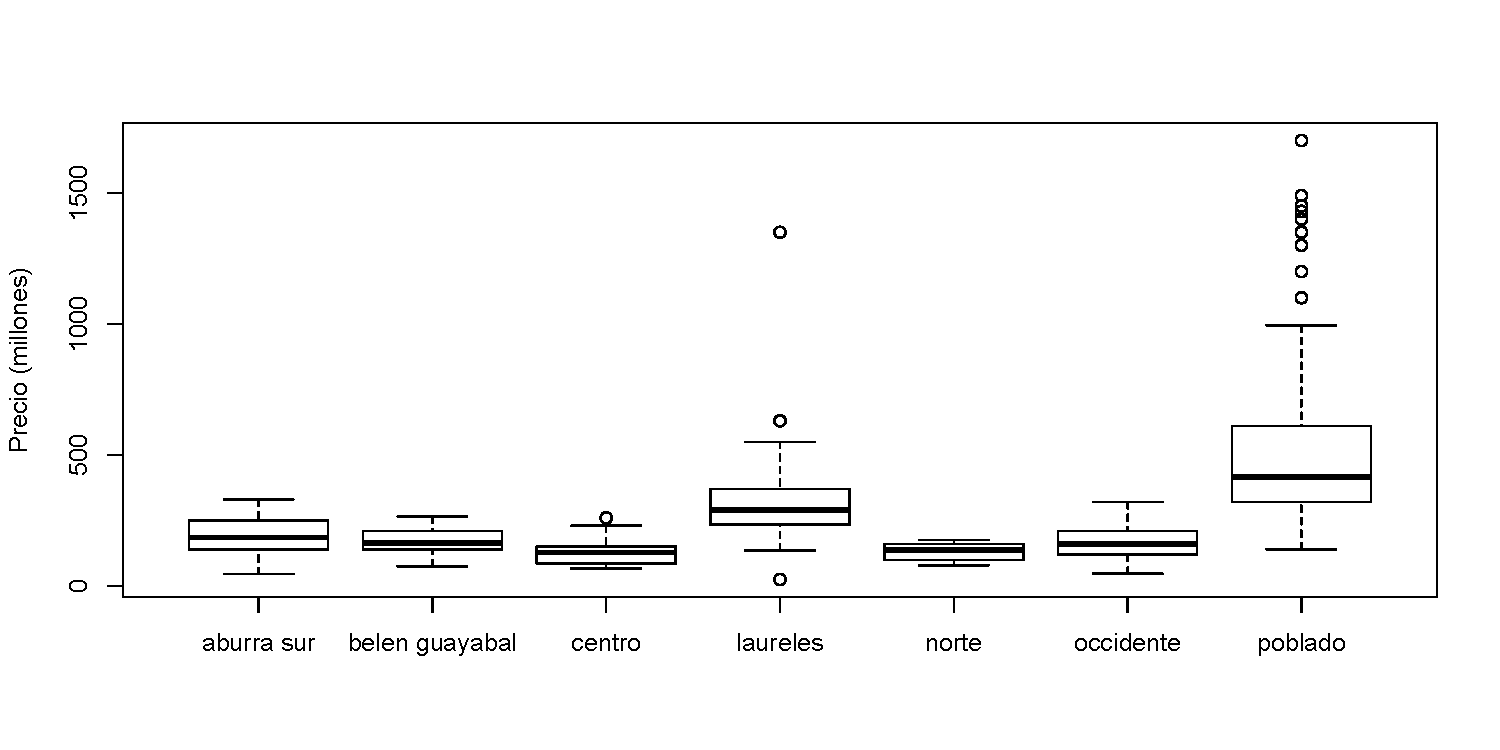
\includegraphics{Manual_de_R_files/figure-latex/box1-1.pdf}
\caption{\label{fig:box1}Boxplot para el precio de los apartamentos dada la
ubicación.}
\end{figure}

\subsection*{Ejemplo}\label{ejemplo-10}


¿Son los resultados de la función \texttt{var} los mismos que los
resultados de la función \texttt{sd} elevados al cuadrado?

La respuesta es \textbf{NO}. La función \texttt{sd} se aplica sólo a
vectores mientras que la función \texttt{var} de puede aplicar tanto a
vectores como a marcos de datos. Al ser aplicada a marcos de datos
numéricos se obtiene una matriz en que la diagonal representa las
varianzas de las de cada una de las variables mientras que arriba y
abajo de la diagonal se encuentran las covarianzas entre pares de
variables.

Por ejemplo, si aplicamos la función \texttt{var} al marco de datos sólo
con las variables precio, área y avaluo se obtiene una matriz de
dimensión \(3 \times 3\), a continuación el código usado.

\begin{Shaded}
\begin{Highlighting}[]
\KeywordTok{var}\NormalTok{(datos[, }\KeywordTok{c}\NormalTok{(}\StringTok{'precio'}\NormalTok{, }\StringTok{'mt2'}\NormalTok{, }\StringTok{'avaluo'}\NormalTok{)])}
\end{Highlighting}
\end{Shaded}

\begin{verbatim}
##        precio   mt2 avaluo
## precio  61313 15874  33056
## mt2     15874  5579   9508
## avaluo  33056  9508  28589
\end{verbatim}

Del anterior resultado se observa la matriz de varianzas y covarianzas
de dimensión \(3 \times 3\).

\section{\texorpdfstring{Coeficiente de variación (\(CV\))
\index{coeficiente de variación}}{Coeficiente de variación (CV) }}\label{coeficiente-de-variacion-cv}

El coeficiente de variación se define como \(CV=s/\bar{x}\) y es muy
sencillo de obtenerlo, la función \texttt{CV} mostrada abajo permite
calcularlo.

\begin{Shaded}
\begin{Highlighting}[]
\NormalTok{CV <-}\StringTok{ }\NormalTok{function(x, }\DataTypeTok{na.rm =} \OtherTok{FALSE}\NormalTok{) \{}
  \KeywordTok{sd}\NormalTok{(x, }\DataTypeTok{na.rm=}\NormalTok{na.rm) /}\StringTok{ }\KeywordTok{mean}\NormalTok{(x, }\DataTypeTok{na.rm=}\NormalTok{na.rm)}
\NormalTok{\}}
\end{Highlighting}
\end{Shaded}

\subsection*{Ejemplo}\label{ejemplo-11}


Calcular el \(CV\) para el vector \texttt{w} definido a continuación.

\begin{Shaded}
\begin{Highlighting}[]
\NormalTok{w <-}\StringTok{ }\KeywordTok{c}\NormalTok{(}\DecValTok{5}\NormalTok{, -}\DecValTok{3}\NormalTok{, }\OtherTok{NA}\NormalTok{, }\DecValTok{8}\NormalTok{, }\DecValTok{8}\NormalTok{, }\DecValTok{7}\NormalTok{)}
\end{Highlighting}
\end{Shaded}

Vemos que el vector \texttt{w} tiene 6 observaciones y la tercera de
ellas es un \texttt{NA}. Lo correcto aquí es usar la función \texttt{CV}
definida antes pero indicándole que remueva los valores faltantes, para
eso se usa el siguiente código.

\begin{Shaded}
\begin{Highlighting}[]
\KeywordTok{CV}\NormalTok{(}\DataTypeTok{x=}\NormalTok{w, }\DataTypeTok{na.rm=}\NormalTok{T)}
\end{Highlighting}
\end{Shaded}

\begin{verbatim}
## [1] 0.9274
\end{verbatim}

\chapter{\texorpdfstring{Medidas de posición
\label{posi}}{Medidas de posición }}\label{medidas-de-posicion}

En este capítulo se mostrará cómo obtener las diferentes medidas de
posición con \proglang{R}.

Para ilustrar el uso de las funciones se utilizará una base de datos
llamada \textbf{medidas del cuerpo}, esta base de datos cuenta con 6
variables registradas a un grupo de 36 estudiantes de la universidad.
Las variables son:

\begin{enumerate}
\def\labelenumi{\arabic{enumi}.}
\tightlist
\item
  \texttt{edad} del estudiante (años),
\item
  \texttt{peso} del estudiante (kilogramos),
\item
  \texttt{altura} del estudiante (centímetros),
\item
  \texttt{sexo} del estudiante (Hombre, Mujer),
\item
  \texttt{muneca}: perímetro de la muñeca derecha (centímetros),
\item
  \texttt{biceps}: perímetro del biceps derecho (centímetros).
\end{enumerate}

A continuación se presenta el código para definir la url donde están los
datos, para cargar la base de datos en R y para mostrar por pantalla un
encabezado (usando \texttt{head}) de la base de datos.

\begin{Shaded}
\begin{Highlighting}[]
\NormalTok{url <-}\StringTok{ 'https://raw.githubusercontent.com/fhernanb/datos/master/medidas_cuerpo'}
\NormalTok{datos <-}\StringTok{ }\KeywordTok{read.table}\NormalTok{(}\DataTypeTok{file=}\NormalTok{url, }\DataTypeTok{header=}\NormalTok{T)}
\KeywordTok{head}\NormalTok{(datos)  }\CommentTok{# Para ver el encabezado de la base de datos}
\end{Highlighting}
\end{Shaded}

\begin{verbatim}
##   edad peso altura   sexo muneca biceps
## 1   43 87.3  188.0 Hombre   12.2   35.8
## 2   65 80.0  174.0 Hombre   12.0   35.0
## 3   45 82.3  176.5 Hombre   11.2   38.5
## 4   37 73.6  180.3 Hombre   11.2   32.2
## 5   55 74.1  167.6 Hombre   11.8   32.9
## 6   33 85.9  188.0 Hombre   12.4   38.5
\end{verbatim}

\section{\texorpdfstring{Cuantiles \index{cuantiles} \index{quantile}
\index{cuartiles} \index{deciles}
\index{percentiles}}{Cuantiles     }}\label{cuantiles}

Para obtener cualquier cuantil (cuartiles, deciles y percentiles) se usa
la función \texttt{quantile}. Los argumentos básicos de la función
\texttt{quantile} son tres y se muestran a continuación.

\begin{Shaded}
\begin{Highlighting}[]
\KeywordTok{quantile}\NormalTok{(x, probs, }\DataTypeTok{na.rm =} \OtherTok{FALSE}\NormalTok{)}
\end{Highlighting}
\end{Shaded}

En el parámetro \texttt{x} se indica la variable de interés para la cual
se quieren calcular los cuantiles, el parámetro \texttt{probs} sirve
para definir los cuantiles de interés y el parámetro \texttt{na.rm} es
un valor lógico que en caso de ser \texttt{TRUE}, significa que se deben
remover las observaciones con \texttt{NA}, el valor por defecto para
este parámetro es \texttt{FALSE}.

\subsection*{Ejemplo}\label{ejemplo-12}


Suponga que queremos obtener el percentil 5, la mediana y el decil 8 pa
la altura del grupo de estudiantes.

Se solicita el percentil 5, la mediana que es el percentil 50 y el decil
8 que corresponde al percentil 80, por lo tanto es necesario indicarle a
la función \texttt{quantile} que calcule los cuantiles para las
ubicaciones 0.05, 0.5 y 0.8, el código para obtener las tres medidas
solicitadas es el siguiente.

\begin{Shaded}
\begin{Highlighting}[]
\KeywordTok{quantile}\NormalTok{(}\DataTypeTok{x=}\NormalTok{datos$altura, }\DataTypeTok{probs=}\KeywordTok{c}\NormalTok{(}\FloatTok{0.05}\NormalTok{, }\FloatTok{0.5}\NormalTok{, }\FloatTok{0.8}\NormalTok{))}
\end{Highlighting}
\end{Shaded}

\begin{verbatim}
##    5%   50%   80% 
## 155.2 172.7 180.3
\end{verbatim}

\chapter{\texorpdfstring{Medidas de correlación
\label{correl}}{Medidas de correlación }}\label{medidas-de-correlacion}

En este capítulo se mostrará cómo obtener las diferentes medidas de

\chapter{Funciones básicas de R}\label{funciones-basicas-de-r}

En este capítulo se presentarán algunas funciones básicas y útiles de
\proglang{R} para realizar diversas tareas.

\section{\texorpdfstring{Operadores de asignación
\index{asignación}}{Operadores de asignación }}\label{operadores-de-asignacion}

En \proglang{R} se pueden hacer asignación de varias formas, a
continuación se presentan los operadores disponibles para tal fin.

\begin{itemize}
\tightlist
\item
  \texttt{\textless{}-}: este es el operador de asignación a izquierda,
  es el más usado y recomendado.
\item
  \texttt{-\textgreater{}}: este es el operador de asignación a derecha,
  no es frecuente su uso.
\item
  \texttt{=}: el símbolo igual sirve para hacer asignaciones pero
  \textbf{NO} se recomienda usarlo.
\item
  \texttt{\textless{}\textless{}-}: este es un operador de asignación
  global y sólo debe ser usado por usuarios avanzados.
\end{itemize}

\subsection*{Ejemplo}\label{ejemplo-13}


Almacene los valores 5.3, 4.6 y 25 en los objetos \texttt{a}, \texttt{b}
y \texttt{age} respectivamente, use diferentes símbolos de asignación.

Para hacer lo solicitado se podría usar el siguiente código.

\begin{Shaded}
\begin{Highlighting}[]
\NormalTok{a <-}\StringTok{ }\FloatTok{5.3} \CommentTok{# Recomended}
\FloatTok{4.6} \NormalTok{->}\StringTok{ }\NormalTok{b }\CommentTok{# It is not usual}
\NormalTok{age =}\StringTok{ }\DecValTok{25} \CommentTok{# Not recomended}
\end{Highlighting}
\end{Shaded}

\section{\texorpdfstring{Operaciones básicas
\index{operaciones básicas}}{Operaciones básicas }}\label{operaciones-basicas}

En \proglang{R} se pueden hacer diversas operaciones usando operadores
binarios. Este tipo de operadores se denomina binarios porque actuan
entre dos objetos, a continuación el listado.

\begin{itemize}
\tightlist
\item
  \texttt{+}: operador binario para sumar.
\item
  \texttt{-}: operador binario para restar.
\item
  \texttt{*}: operador binario para multiplicar.
\item
  \texttt{/}: operador binario para dividir.
\item
  \texttt{\^{}}: operador binario para potencia.
\item
  \texttt{\%/\%}: operador binario para obtener el cociente en una
  división (número entero).
\item
  \texttt{\%\%}: operador binario para obtener el residuo en una
  división.
\end{itemize}

A continuación se presentan ejemplos de cómo usar las anteriores
funciones.

\begin{Shaded}
\begin{Highlighting}[]
\DecValTok{6} \NormalTok{+}\StringTok{ }\DecValTok{4}  \CommentTok{# Para sumar dos números}
\end{Highlighting}
\end{Shaded}

\begin{verbatim}
## [1] 10
\end{verbatim}

\begin{Shaded}
\begin{Highlighting}[]
\NormalTok{a <-}\StringTok{ }\KeywordTok{c}\NormalTok{(}\DecValTok{1}\NormalTok{, }\DecValTok{3}\NormalTok{, }\DecValTok{2}\NormalTok{)}
\NormalTok{b <-}\StringTok{ }\KeywordTok{c}\NormalTok{(}\DecValTok{2}\NormalTok{, }\DecValTok{0}\NormalTok{, }\DecValTok{1}\NormalTok{)  }\CommentTok{# a y b de la misma dimensión}
\NormalTok{a +}\StringTok{ }\NormalTok{b  }\CommentTok{# Para sumar los vectores a y b miembro a miembro}
\end{Highlighting}
\end{Shaded}

\begin{verbatim}
## [1] 3 3 3
\end{verbatim}

\begin{Shaded}
\begin{Highlighting}[]
\NormalTok{a -}\StringTok{ }\NormalTok{b  }\CommentTok{# Para restar dos vectores a y b miembro a miembro}
\end{Highlighting}
\end{Shaded}

\begin{verbatim}
## [1] -1  3  1
\end{verbatim}

\begin{Shaded}
\begin{Highlighting}[]
\NormalTok{a *}\StringTok{ }\NormalTok{b  }\CommentTok{# Para multiplicar}
\end{Highlighting}
\end{Shaded}

\begin{verbatim}
## [1] 2 0 2
\end{verbatim}

\begin{Shaded}
\begin{Highlighting}[]
\NormalTok{a /}\StringTok{ }\NormalTok{b  }\CommentTok{# Para dividir}
\end{Highlighting}
\end{Shaded}

\begin{verbatim}
## [1] 0.5 Inf 2.0
\end{verbatim}

\begin{Shaded}
\begin{Highlighting}[]
\NormalTok{a ^}\StringTok{ }\NormalTok{b  }\CommentTok{# Para potencia}
\end{Highlighting}
\end{Shaded}

\begin{verbatim}
## [1] 1 1 2
\end{verbatim}

\begin{Shaded}
\begin{Highlighting}[]
\DecValTok{7} \NormalTok\StringTok{ }\DecValTok{3}  \CommentTok{# Para saber las veces que cabe 3 en 7}
\end{Highlighting}
\end{Shaded}

\begin{verbatim}
## [1] 2
\end{verbatim}

\begin{Shaded}
\begin{Highlighting}[]
\DecValTok{7} \NormalTok\StringTok{ }\DecValTok{3}  \CommentTok{# Para saber el residuo al dividir 7 entre 3}
\end{Highlighting}
\end{Shaded}

\begin{verbatim}
## [1] 1
\end{verbatim}

\section{\texorpdfstring{Pruebas lógicas
\index{pruebas lógicas}}{Pruebas lógicas }}\label{pruebas-logicas}

En \proglang{R} se puede verificar si un objeto cumple una condición
dada, a continuación el listado de las pruebas usuales.

\begin{itemize}
\tightlist
\item
  \texttt{\textless{}}: para saber si un número es menor que otro.
\item
  \texttt{\textgreater{}}: para saber si un número es mayor que otro.
\item
  \texttt{==}: para saber si un número es igual que otro.
\item
  \texttt{\textless{}=}: para saber si un número es menor o igual que
  otro.
\item
  \texttt{\textgreater{}=}: para saber si un número es mayor o igual que
  otro.
\end{itemize}

A continuación se presentan ejemplos de cómo usar las anteriores
funciones.

\begin{Shaded}
\begin{Highlighting}[]
\DecValTok{5} \NormalTok{<}\StringTok{ }\DecValTok{12}  \CommentTok{# ¿Será 5 menor que 12?}
\end{Highlighting}
\end{Shaded}

\begin{verbatim}
## [1] TRUE
\end{verbatim}

\begin{Shaded}
\begin{Highlighting}[]
\CommentTok{# Comparando objetos}
\NormalTok{x <-}\StringTok{ }\DecValTok{5}
\NormalTok{y <-}\StringTok{ }\DecValTok{20} \NormalTok{/}\StringTok{ }\DecValTok{4}
\NormalTok{x ==}\StringTok{ }\NormalTok{y  }\CommentTok{# ¿Será x igual a y?}
\end{Highlighting}
\end{Shaded}

\begin{verbatim}
## [1] TRUE
\end{verbatim}

\begin{Shaded}
\begin{Highlighting}[]
\CommentTok{# Usando vectores}
\NormalTok{a <-}\StringTok{ }\KeywordTok{c}\NormalTok{(}\DecValTok{1}\NormalTok{, }\DecValTok{3}\NormalTok{, }\DecValTok{2}\NormalTok{)}
\NormalTok{b <-}\StringTok{ }\KeywordTok{c}\NormalTok{(}\DecValTok{2}\NormalTok{, }\DecValTok{0}\NormalTok{, }\DecValTok{1}\NormalTok{)}
\NormalTok{a >}\StringTok{ }\NormalTok{b  }\CommentTok{# Comparación término a término}
\end{Highlighting}
\end{Shaded}

\begin{verbatim}
## [1] FALSE  TRUE  TRUE
\end{verbatim}

\begin{Shaded}
\begin{Highlighting}[]
\NormalTok{a ==}\StringTok{ }\NormalTok{b  }\CommentTok{# Comparación de igualdad término a término}
\end{Highlighting}
\end{Shaded}

\begin{verbatim}
## [1] FALSE FALSE FALSE
\end{verbatim}

\subsection*{Ejemplo}\label{ejemplo-14}


Crear un vector con los números de 1 a 17 y extrater los números que son
mayores o iguales a 12.

Primero se crear el vector \texttt{x} con los elementos del 1 al 17. La
prueba lógica \texttt{x\ \textgreater{}=\ 12} se usa para evaluar la
condición, el resultado es un vector de 17 posiciones con valores de
\texttt{TRUE} o \texttt{FALSE} dependiendo de si la condición se cumple
o no. Este vector lógico se coloca dentro de \texttt{x{[}\ {]}} para que
al evaluar \texttt{x{[}x\ \textgreater{}=\ 12{]}} sólo aparezcan los
valores del vector original que SI cumplen la condición. El código
necesario se muestra a continuación.

\begin{Shaded}
\begin{Highlighting}[]
\NormalTok{x <-}\StringTok{ }\DecValTok{1}\NormalTok{:}\DecValTok{17}  \CommentTok{# Se crea el vector}
\NormalTok{x[x >=}\StringTok{ }\DecValTok{12}\NormalTok{]  }\CommentTok{# Se solicitan los valores que cumplen la condición}
\end{Highlighting}
\end{Shaded}

\begin{verbatim}
## [1] 12 13 14 15 16 17
\end{verbatim}

\section{\texorpdfstring{Operadores lógicos
\index{operadores lógicos}}{Operadores lógicos }}\label{operadores-logicos}

En \proglang{R} están disponibles los operadores lógicos negación,
conjunción y disyunción. A continuación el listado de los operadores
entre los elementos \texttt{x} e \texttt{y}.

\begin{Shaded}
\begin{Highlighting}[]
\NormalTok{!x  }\CommentTok{# Negación de x}
\NormalTok{x &}\StringTok{ }\NormalTok{y  }\CommentTok{# Conjunción entre x e y}
\NormalTok{x &&}\StringTok{ }\NormalTok{y}
\NormalTok{x |}\StringTok{ }\NormalTok{y  }\CommentTok{# Disyunción entre x e y}
\NormalTok{x ||}\StringTok{ }\NormalTok{y}
\KeywordTok{xor}\NormalTok{(x, y)}
\end{Highlighting}
\end{Shaded}

A continuación se presentan ejemplos de cómo usar el símbolo de negación
\texttt{!}.

\begin{Shaded}
\begin{Highlighting}[]
\NormalTok{ans <-}\StringTok{ }\KeywordTok{c}\NormalTok{(}\OtherTok{TRUE}\NormalTok{, }\OtherTok{FALSE}\NormalTok{, }\OtherTok{TRUE}\NormalTok{)}
\NormalTok{!ans  }\CommentTok{# Negando las respuestas almacenadas en ans}
\end{Highlighting}
\end{Shaded}

\begin{verbatim}
## [1] FALSE  TRUE FALSE
\end{verbatim}

\begin{Shaded}
\begin{Highlighting}[]
\NormalTok{x <-}\StringTok{ }\KeywordTok{c}\NormalTok{(}\DecValTok{5}\NormalTok{, }\FloatTok{1.5}\NormalTok{, }\DecValTok{2}\NormalTok{, }\DecValTok{3}\NormalTok{, }\DecValTok{2}\NormalTok{)}
\NormalTok{!(x <}\StringTok{ }\FloatTok{2.5}\NormalTok{)  }\CommentTok{# Negando los resultados de una prueba}
\end{Highlighting}
\end{Shaded}

\begin{verbatim}
## [1]  TRUE FALSE FALSE  TRUE FALSE
\end{verbatim}

A continuación se presentan ejemplos de cómo aplicar la conjunción
\texttt{\&} y \texttt{\&\&}.

\begin{Shaded}
\begin{Highlighting}[]
\NormalTok{x <-}\StringTok{ }\KeywordTok{c}\NormalTok{(}\DecValTok{5}\NormalTok{, }\FloatTok{1.5}\NormalTok{, }\DecValTok{2}\NormalTok{)  }\CommentTok{# Se construyen dos vectores para la prueba}
\NormalTok{y <-}\StringTok{ }\KeywordTok{c}\NormalTok{(}\DecValTok{4}\NormalTok{, }\DecValTok{6}\NormalTok{, }\DecValTok{3}\NormalTok{)}

\NormalTok{x <}\StringTok{ }\DecValTok{4}  \CommentTok{# ¿Serán los elementos de x menores que 4?}
\end{Highlighting}
\end{Shaded}

\begin{verbatim}
## [1] FALSE  TRUE  TRUE
\end{verbatim}

\begin{Shaded}
\begin{Highlighting}[]
\NormalTok{y >}\StringTok{ }\DecValTok{5}  \CommentTok{# ¿Serán los elementos de y mayores que 5?}
\end{Highlighting}
\end{Shaded}

\begin{verbatim}
## [1] FALSE  TRUE FALSE
\end{verbatim}

\begin{Shaded}
\begin{Highlighting}[]
\NormalTok{x <}\StringTok{ }\DecValTok{4} \NormalTok{&}\StringTok{ }\NormalTok{y >}\StringTok{ }\DecValTok{5}  \CommentTok{# Conjunción entre las pruebas anteriores.}
\end{Highlighting}
\end{Shaded}

\begin{verbatim}
## [1] FALSE  TRUE FALSE
\end{verbatim}

\begin{Shaded}
\begin{Highlighting}[]
\NormalTok{x <}\StringTok{ }\DecValTok{4} \NormalTok{&&}\StringTok{ }\NormalTok{y >}\StringTok{ }\DecValTok{5}  \CommentTok{# Conjunción vectorial}
\end{Highlighting}
\end{Shaded}

\begin{verbatim}
## [1] FALSE
\end{verbatim}

Note las diferencias entre los dos últimos ejemplos, cuando se usa
\texttt{\&} se hace una prueba término a término y el resultado es un
vector, cuando se usa \texttt{\&\&} se aplica la conjunción al vector de
resultados obtenido con \texttt{\&}.

\section{Funciones sobre vectores}\label{funciones-sobre-vectores}

En \proglang{R} podemos destacar las siguientes funciones básicas sobre
vectores numéricos.

\begin{itemize}
\tightlist
\item
  \texttt{min}: para obtener el mínimo de un vector.
\item
  \texttt{max}: para obtener el máximo de un vector.
\item
  \texttt{length}: para determinar la longitud de un vector.
\item
  \texttt{range}: para obtener el rango de valores de un vector, entrega
  el mínimo y máximo.
\item
  \texttt{sum}: entrega la suma de todos los elementos del vector.
\item
  \texttt{prod}: multiplica todos los elementos del vector.
\item
  \texttt{which.min}: nos entrega la posición en donde está el valor
  mínimo del vector.
\item
  \texttt{which.max}: nos da la posición del valor máximo del vector.
\end{itemize}

\subsection*{Ejemplo}\label{ejemplo-15}


Construir en vector llamado \texttt{myvec} con los siguientes elementos:
5, 3, 2, 1, 2, 0, NA, 0, 9, 6. Luego aplicar todas las funciones
anteriores para verificar el funcionamiento de las mismas.

\begin{Shaded}
\begin{Highlighting}[]
\NormalTok{myvec <-}\StringTok{ }\KeywordTok{c}\NormalTok{(}\DecValTok{5}\NormalTok{, }\DecValTok{3}\NormalTok{, }\DecValTok{2}\NormalTok{, }\DecValTok{1}\NormalTok{, }\DecValTok{2}\NormalTok{, }\DecValTok{0}\NormalTok{, }\OtherTok{NA}\NormalTok{, }\DecValTok{0}\NormalTok{, }\DecValTok{9}\NormalTok{, }\DecValTok{6}\NormalTok{)}
\NormalTok{myvec}
\end{Highlighting}
\end{Shaded}

\begin{verbatim}
##  [1]  5  3  2  1  2  0 NA  0  9  6
\end{verbatim}

\begin{Shaded}
\begin{Highlighting}[]
\KeywordTok{min}\NormalTok{(myvec)  }\CommentTok{# Opss, no aparece el mínimo que es Cero.}
\end{Highlighting}
\end{Shaded}

\begin{verbatim}
## [1] NA
\end{verbatim}

\begin{Shaded}
\begin{Highlighting}[]
\KeywordTok{min}\NormalTok{(myvec, }\DataTypeTok{na.rm=}\OtherTok{TRUE}\NormalTok{)  }\CommentTok{# Usamos na.rm = TRUE para remover el NA}
\end{Highlighting}
\end{Shaded}

\begin{verbatim}
## [1] 0
\end{verbatim}

\begin{Shaded}
\begin{Highlighting}[]
\KeywordTok{max}\NormalTok{(myvec, }\DataTypeTok{na.rm=}\NormalTok{T)  }\CommentTok{# Para obtener el valor máximo}
\end{Highlighting}
\end{Shaded}

\begin{verbatim}
## [1] 9
\end{verbatim}

\begin{Shaded}
\begin{Highlighting}[]
\KeywordTok{range}\NormalTok{(myvec, }\DataTypeTok{na.rm=}\NormalTok{T)  }\CommentTok{# Genera min y max simultáneamente}
\end{Highlighting}
\end{Shaded}

\begin{verbatim}
## [1] 0 9
\end{verbatim}

\begin{Shaded}
\begin{Highlighting}[]
\KeywordTok{sum}\NormalTok{(myvec, }\DataTypeTok{na.rm=}\NormalTok{T)  }\CommentTok{# La suma de los valores internos}
\end{Highlighting}
\end{Shaded}

\begin{verbatim}
## [1] 28
\end{verbatim}

\begin{Shaded}
\begin{Highlighting}[]
\KeywordTok{prod}\NormalTok{(myvec, }\DataTypeTok{na.rm=}\NormalTok{T)  }\CommentTok{# El productor de los valores internos}
\end{Highlighting}
\end{Shaded}

\begin{verbatim}
## [1] 0
\end{verbatim}

\begin{Shaded}
\begin{Highlighting}[]
\KeywordTok{which.min}\NormalTok{(myvec)  }\CommentTok{# Posición del valor mínimo 0 en el vector}
\end{Highlighting}
\end{Shaded}

\begin{verbatim}
## [1] 6
\end{verbatim}

\begin{Shaded}
\begin{Highlighting}[]
\KeywordTok{which.max}\NormalTok{(myvec)  }\CommentTok{# Posición del valor máximo 9 en el vector}
\end{Highlighting}
\end{Shaded}

\begin{verbatim}
## [1] 9
\end{verbatim}

De las dos últimas líneas podemos destacar lo siguiente:

\begin{enumerate}
\def\labelenumi{\arabic{enumi}.}
\tightlist
\item
  \textbf{NO es necesario} usar \texttt{na.rm\ =\ TRUE} para remover el
  \texttt{NA} dentro de las funciones \texttt{which.min} ni
  \texttt{which.max}.
\item
  El valor mínimo 0 aparece en las posiciones 6 y 8 pero la función
  \texttt{which.min} sólo entrega la posición del primer valor mínimo
  dentro del vector.
\end{enumerate}

\section*{EJERCICIOS}\label{ejercicios}


Use funciones o procedimientos (varias líneas) de \proglang{R} para
responder cada una de las siguientes preguntas.

\begin{enumerate}
 \item ¿Qué cantidad de dinero sobra al repartir 10000\$ entre 3 personas?
 \item ¿Es el número 4560 divisible por 3?
 \item Construya un vector con los números enteros del 2 al 87. ¿Cuáles de esos números son divisibles por 7?
 \item Construya dos vectores, el primero con los números enteros desde 7 hasta 3, el segundo vector con los primeros cinco números positivos divisibles por 5. Sea A la condición de ser par en el primer vector. Sea B la condición de ser mayor que 10 en el segundo vector. ¿En cuál de las 5 posiciones se cumple A y B simultáneamente?
 \item Construya un vector con los siguientes elementos: 1, -4, 5, 9, -4. Escriba un procedimiento para extraer las posiciones donde está el valor mínimo en el vector.
\end{enumerate}

\chapter{\texorpdfstring{Creación de funciones en
\proglang{R}}{Creación de funciones en }}\label{creacion-de-funciones-en}

En este capítulo se

\chapter{Distribuciones discretas}\label{distribuciones-discretas}

En este capítulo se

\chapter{Distribuciones continuas}\label{distribuciones-continuas}

En este capítulo se

\chapter{Pruebas de bondad de ajuste}\label{pruebas-de-bondad-de-ajuste}

En este capítulo se

\chapter{Aproximación de integrales}\label{aproximacion-de-integrales}

En este capítulo se mostrará cómo aproximar integrales en una y varias
dimensiones.

\section{Aproximación de Laplace
unidimensional}\label{aproximacion-de-laplace-unidimensional}

Esta aproximación es útil para obtener el valor de una integral usando
la expansión de Taylor para una función \(f(x)\) unimodal en \(\Re\), en
otras palabras lo que interesa es:
\[ I = \int_{-\infty}^{\infty} f(x) d(x)\] Al hacer una expansión de
Taylor de segundo orden para \(\log(f(x))\) en su moda \(x_0\) el
resultado es:
\[ \log(f(x)) \approx \log(f(x_0)) + \frac{\log(f)^\prime(x_0)}{1!} (x-x_0) + \frac{\log(f)^{\prime \prime}(x_0)}{2!} (x-x_0)^2 \]
El segundo término de la suma se anula porque \(\log(f)^\prime(x_0)=0\)
por ser \(x_0\) el valor donde está el máximo de \(\log(f(x))\). La
expresión anterior se simplifica en:
\[ \log(f(x)) \approx \log(f(x_0)) + \frac{\log(f)^{\prime \prime}(x_0)}{2!} (x-x_0)^2 \]
al aislar \(f(x)\) se tiene que

\begin{equation} \label{fx}
f(x) \approx f(x_0)  \exp \left( -\frac{c}{2} (x-x_0)^2 \right)
\end{equation}

donde \(c=-\frac{d^2}{dx^2} \log(f(x)) \bigg|_{x=x_0}\).

La expresión \ref{fx} se puede reescribir de manera que aparezca el
núcleo de la función de densidad de la distribución normal con media
\(x_0\) y varianza \(1/c\), a continuación la expresión

\[
f(x) \approx f(x_0) \frac{\sqrt{2 \pi / c}}{\sqrt{2 \pi / c}}  \exp \left( -\frac{1}{2} \left( \frac{x-x_0}{1/\sqrt{c}} \right)^2 \right)
\] Así al calcular la integral de \(f(x)\) en \(\Re\) se tiene que:

\begin{equation} \label{aprox_laplace}
I = \int_{-\infty}^{\infty} f(x) d(x) = f(x_0) \sqrt{2 \pi / c}
\end{equation}

\subsection*{Ejemplo}\label{ejemplo-16}


Calcular la integral de \(f(x)=\exp \left( -(x-1.5)^2 \right)\) en
\(\Re\) utilizando la aproximación de Laplace.

Primero vamos a dibujar la función \(f(x)\) para ver en dónde está su
moda \(x_0\).

\begin{Shaded}
\begin{Highlighting}[]
\NormalTok{fun <-}\StringTok{ }\NormalTok{function(x) }\KeywordTok{exp}\NormalTok{(-(x}\FloatTok{-1.5}\NormalTok{)^}\DecValTok{2}\NormalTok{)}
\KeywordTok{curve}\NormalTok{(fun, }\DataTypeTok{from=}\NormalTok{-}\DecValTok{5}\NormalTok{, }\DataTypeTok{to=}\DecValTok{5}\NormalTok{, }\DataTypeTok{ylab=}\StringTok{'f(x)'}\NormalTok{, }\DataTypeTok{las=}\DecValTok{1}\NormalTok{)}
\end{Highlighting}
\end{Shaded}

\begin{figure}[htbp]
\centering
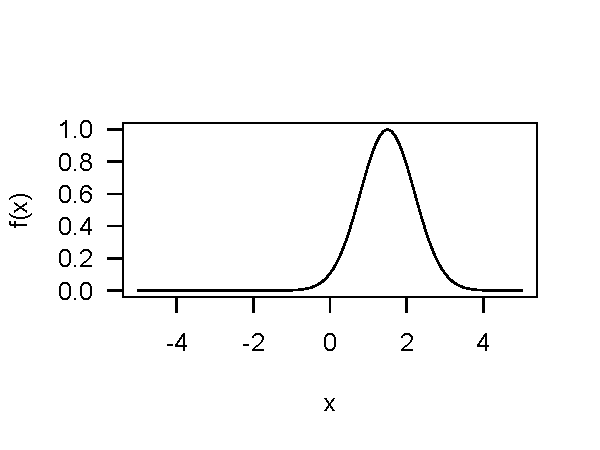
\includegraphics{Manual_de_R_files/figure-latex/unnamed-chunk-59-1.pdf}
\caption{\label{fig:unnamed-chunk-59}Perfil de la función f(x).}
\end{figure}

Visualmente se nota que la moda está cerca del valor 1.5 y para
determinar numéricamente el valor de la moda \(x_0\) se usa la función
\texttt{optimize}, los resultados se almacenan en el objeto
\texttt{res}. El valor de la moda corresponde al elemento
\texttt{maximum} del objeto \texttt{res}.

\begin{Shaded}
\begin{Highlighting}[]
\NormalTok{res <-}\StringTok{ }\KeywordTok{optimize}\NormalTok{(fun, }\DataTypeTok{interval=}\KeywordTok{c}\NormalTok{(-}\DecValTok{10}\NormalTok{, }\DecValTok{10}\NormalTok{), }\DataTypeTok{maximum=}\OtherTok{TRUE}\NormalTok{)}
\NormalTok{res}
\end{Highlighting}
\end{Shaded}

\begin{verbatim}
## $maximum
## [1] 1.5
## 
## $objective
## [1] 1
\end{verbatim}

Para determinar el valor de \(c\) de la expresión \ref{aprox_laplace} se
utiliza el siguiente código.

\begin{Shaded}
\begin{Highlighting}[]
\KeywordTok{require}\NormalTok{(}\StringTok{"numDeriv"}\NormalTok{)}
\NormalTok{constant <-}\StringTok{ }\NormalTok{-}\StringTok{ }\KeywordTok{as.numeric}\NormalTok{(}\KeywordTok{hessian}\NormalTok{(fun, res$maximum))}
\end{Highlighting}
\end{Shaded}

Para obtener la aproximación de la integral se usa la expresión
\ref{aprox_laplace} y para tener un punto de comparación se evalua la
integral usando la función \texttt{integrate}, a continuación el código.

\begin{Shaded}
\begin{Highlighting}[]
\KeywordTok{fun}\NormalTok{(res$maximum) *}\StringTok{ }\KeywordTok{sqrt}\NormalTok{(}\DecValTok{2}\NormalTok{*pi/constant)}
\end{Highlighting}
\end{Shaded}

\begin{verbatim}
## [1] 1.772
\end{verbatim}

\begin{Shaded}
\begin{Highlighting}[]
\KeywordTok{integrate}\NormalTok{(fun, -}\OtherTok{Inf}\NormalTok{, }\OtherTok{Inf}\NormalTok{)  }\CommentTok{# Para comparar}
\end{Highlighting}
\end{Shaded}

\begin{verbatim}
## 1.772 with absolute error < 1.5e-06
\end{verbatim}

De los anteriores resultados vemos que la aproximación es buena.

\bibliography{packages,book}

\backmatter
\printindex

\end{document}
